\documentclass[compsoc, conference, a4paper, 10pt, times]{IEEEtran}
% \IEEEoverridecommandlockouts
% The preceding line is only needed to identify funding in the first footnote. If that is unneeded, please comment it out.
% \usepackage{cite}
%\usepackage{amsmath,amssymb,amsfonts}

% \settopmatter{printfolios=true}  % page numbers
% \settopmatter{printacmref=false} % removes citation information below abstract
% \renewcommand\footnotetextcopyrightpermission[1]{} % removes footnote with confe

\usepackage{algorithmic}
\usepackage{graphicx}
\usepackage{textcomp}
\usepackage{xcolor}
\usepackage{colortbl} % using this in lieu of xcolor because xcolor was erroring
%\usepackage{usenix}
\usepackage{subcaption}
\usepackage{caption}
\captionsetup[table]{skip=10pt}
\usepackage{xspace}
\usepackage{booktabs}
\usepackage{amssymb}
\usepackage{multirow}
\usepackage{diagbox}
\usepackage[flushleft]{threeparttable}
\usepackage{scalerel}
\usepackage{tikz}
\usetikzlibrary{svg.path}

\definecolor{orcidlogocol}{HTML}{A6CE39}
\tikzset{
  orcidlogo/.pic={
    \fill[orcidlogocol] svg{M256,128c0,70.7-57.3,128-128,128C57.3,256,0,198.7,0,128C0,57.3,57.3,0,128,0C198.7,0,256,57.3,256,128z};
    \fill[white] svg{M86.3,186.2H70.9V79.1h15.4v48.4V186.2z}
                 svg{M108.9,79.1h41.6c39.6,0,57,28.3,57,53.6c0,27.5-21.5,53.6-56.8,53.6h-41.8V79.1z M124.3,172.4h24.5c34.9,0,42.9-26.5,42.9-39.7c0-21.5-13.7-39.7-43.7-39.7h-23.7V172.4z}
                 svg{M88.7,56.8c0,5.5-4.5,10.1-10.1,10.1c-5.6,0-10.1-4.6-10.1-10.1c0-5.6,4.5-10.1,10.1-10.1C84.2,46.7,88.7,51.3,88.7,56.8z};
  }
}

\newcommand\orcidicon[1]{\href{https://orcid.org/#1}{\mbox{\scalerel*{

\begin{tikzpicture}[yscale=-1,transform shape]
\pic{orcidlogo};
\end{tikzpicture}
}{|}}}}

\usepackage{hyperref}
\newcommand{\dns}[1]{{\small \texttt{#1}}}
\newcommand{\dnsfn}[1]{{\footnotesize \texttt{#1}}}
\newcommand{\foo}{\dns{foo.com}\xspace}
\newcommand{\ie}{i.e.}
\newcommand{\eg}{e.g.}
\newcommand{\etal}{et al.}

\def\BibTeX{{\rm B\kern-.05em{\sc i\kern-.025em b}\kern-.08em
    T\kern-.1667em\lower.7ex\hbox{E}\kern-.125emX}}


% Change \paragraph spacing
\renewcommand{\paragraph}[1]{\vspace{5pt}\noindent\textbf{#1:}}

% \copyrightyear{2022}
% \acmYear{2022}
% \acmConference[IMC '22]{Internet Measurement Conference}{October 25--27, 2022}{Nice, France}
% \acmBooktitle{Internet Measurement Conference (IMC '22), October 25--27, 2022, Nice, France}
%\acmPrice{TBA}
\newcommand{\ltgrey}{\rowcolor[gray]{0.95}}
\definecolor{chicagomaroon}{rgb}{0.5, 0.0, 0.0}
\definecolor{midgreen}{rgb}{0.0, 0.50, 0.0}

\makeatletter
% \newcommand*\titleheader[1]{\gdef\@titleheader{#1}}
% \AtBeginDocument{%
%   \let\st@red@title\@title
%   \def\@title{%
%     \bgroup\normalfont\large\centering\@titleheader\par\egroup
%     \vskip1.5em\st@red@title}
% }
\newcommand{\linebreakand}{%
  \end{@IEEEauthorhalign}
  \hfill\mbox{}\par
  \mbox{}\hfill\begin{@IEEEauthorhalign}
}
\makeatother

\title{
  Forward Pass: On the Security Implications of\\Email Forwarding Mechanism and Policy\\
}
% \titleheader{This is a preprint of a paper to appear at the 8th IEEE European Symposium on Security and Privacy }

\begin{document}



% \iffalse
% \newcommand{\grant}[1]{\textsf{\textcolor{teal}{[GH: #1]}}}
% \newcommand{\gakiwate}[1]{\textcolor{violet}{\noindent[Gautam: #1]}}
% \newcommand{\geoff}[1]{\textcolor{purple}{\noindent[GV: #1]}}
% \newcommand{\stefan}[1]{\textcolor{green}{\noindent[SS: #1]}}
% \newcommand{\mattijs}[1]{\textcolor{blue}{\noindent[MJ: #1]}}
% \newcommand{\alex}[1]{\textcolor{chicagomaroon}{\noindent[AL: #1]}}
% \else
% \newcommand{\grant}[1]{}
% \newcommand{\gakiwate}[1]{}
% \newcommand{\geoff}[1]{}
% \newcommand{\stefan}[1]{}
% \newcommand{\mattijs}[1]{}
% \newcommand{\alex}[1]{}
% \fi

\iffalse

\newcommand{\todo}[1]{\textsf{\textcolor{red}{[TODO: #1]}}}
\newcommand{\grant}[1]{\textsf{\textcolor{teal}{[GH: #1]}}}
\newcommand{\amirian}[1]{\textsf{\textcolor{violet}{[AM: #1]}}}
\newcommand{\gakiwate}[1]{\textcolor{violet}{\noindent[Gautam: #1]}}
\newcommand{\geoff}[1]{\textcolor{purple}{\noindent[GV: #1]}}
\newcommand{\stefan}[1]{\textcolor{green}{\noindent[SS: #1]}}
\newcommand{\mattijs}[1]{\textcolor{blue}{\noindent[MJ: #1]}}
\newcommand{\alex}[1]{\textcolor{chicagomaroon}{\noindent[AL: #1]}}
\else
\newcommand{\todo}[1]{}
\newcommand{\amirian}[1]{}
\newcommand{\grant}[1]{}
\newcommand{\gakiwate}[1]{}
\newcommand{\geoff}[1]{}
\newcommand{\stefan}[1]{}
\newcommand{\mattijs}[1]{}
\newcommand{\alex}[1]{}
\fi





\author{
\IEEEauthorblockN{Enze Liu \orcidicon{0000-0003-4288-8485}}
  \IEEEauthorblockA{
  \textit{UC San Diego}\\
  La Jolla, CA, USA \\
  e7liu@eng.ucsd.edu}
\and
\IEEEauthorblockN{Gautam Akiwate}
\IEEEauthorblockA{
\textit{Stanford University}\\
Stanford, CA, USA \\
gakiwate@cs.stanford.edu}
\and
\IEEEauthorblockN{Mattijs Jonker}
\IEEEauthorblockA{
\textit{University of Twente}\\
Enschede, Netherlands \\
m.jonker@utwente.nl}
\and
\IEEEauthorblockN{Ariana Mirian}
\IEEEauthorblockA{
\textit{UC San Diego}\\
La Jolla, CA, USA \\
amirian@cs.ucsd.edu}\\
\linebreakand
\IEEEauthorblockN{Grant Ho}
\IEEEauthorblockA{
\textit{UC San Diego}\\
La Jolla, CA, USA \\
grho@eng.ucsd.edu}
\and
\IEEEauthorblockN{Geoffrey M. Voelker}
\IEEEauthorblockA{
\textit{UC San Diego}\\
La Jolla, CA, USA \\
voelker@cs.ucsd.edu}
\and
\IEEEauthorblockN{Stefan Savage}
\IEEEauthorblockA{
\textit{UC San Diego}\\
La Jolla, CA, USA \\
savage@cs.ucsd.edu}\\
}

\maketitle

\begin{abstract}
The critical role played by email has led to a range of extension
protocols (\eg, SPF, DKIM, DMARC) designed to protect against the
spoofing of email sender domains.  These protocols are complex as is,
but are further complicated by automated email forwarding --- used by
individual users to manage multiple accounts and by mailing lists to
redistribute messages.  In this paper, we explore how such email
forwarding and its implementations can break the implicit assumptions
in widely deployed anti-spoofing protocols.  Using large-scale empirical
measurements of 20 email forwarding services (16 leading email providers and four popular mailing
list services), we identify a range of security issues rooted in
forwarding behavior and show how they can be combined to reliably
evade existing anti-spoofing controls.  We further show how these issues allow
attackers to not only deliver spoofed email messages to prominent email providers (e.g., Gmail, Microsoft Outlook, and Zoho), but also reliably spoof email on behalf of tens of thousands of
popular domains including sensitive domains used by organizations in
government (\eg, \dns{state.gov}), finance (\eg, \dns{transunion.com}), law (\eg,
\dns{perkinscoie.com}) and news (\eg, \dns{washingtonpost.com}) among others.

%%on the deployment of e-mail forwarding mechanisms and the
%%treatment of forwarded e-mail messages by studying six prominent
%%e-mail providers and four popular mailing list software. We first
%%document how e-mail forwarding is implemented in the wild and how
%%forwarded e-mail messages are handled. We identify X security
%%vulnerabilities among parties involved in the forwarding flow. Using a
%%combination of these vulnerabilities, we show 5 types of evasion
%%exploits that affect leading e-mail service providers (\eg, Gmail,
%%Microsoft Outlook and Zoho) and mailing list providers/software (\eg,
%%Google Groups and Gaggle.email). We demonstrate with a large-scale DNS
%%measurement to quantify the impact of these exploits.

% E-mail has long been a critical component of daily communication. As with many pieces of key communications infrastructures, increasingly this function has been outsourced to a few major third-party e-mail service providers. Such centralization also buries implicit trust in these provider. On the one hand, these providers are assumed to defend against various spoofing and phishing attacks. Failing to do so can cause serious harms to their users. The prevalence of mailing lists further amplifies this concern, as they make the distribution of malicious e-mail messages easier. On the other hand, certain providers might trust other providers in that others have done their due diligence in combating various attacks, which might not always be the case.

% In this paper, we show that such trust can be violated and abused by an adversary who leverages e-mail forwarding. Our key findings are three fold. First, we document how e-mail forwarding is carried out in the wild by studying six prominent e-mail providers and four popular mailing lists. Second, we characterize implicit trust in each provider and between providers. Finally, we show how such trust can be abused in the presence of an adversary.

% This paper performs the first empirical study that documents e-mail forwarding practices in the wild and security risks that exist. We examine forwarding mechanisms used by six prominent e-mail providers and four popular mailing list software. We also identify X security exploits among those providers and software. Using a combination of these exploits, we
% demonstrate 5 types of evasion exploits that affect leading e-mail service providers such as Google and Microsoft.

% Due to its nature, it break SPF
% It's thus handled differently with Assumptions made
% previous work not comprehensive
% no work on assumptions.

% Despite being useful, e-mail for- warding also raises security concerns due to various assump- tions made by different parties involved. Such assumptions, when coupled with specific implementation, can easily be violated. While past literature has shed light on the possibility of abusing e-mail forwarding, there has been little compre- hensive work on how e-mail forwarding is implemented in practice and what assumptions are being made by each party.

\end{abstract}


%\begin{abstract}
The critical role played by email has led to a range of extension
protocols (\eg, SPF, DKIM, DMARC) designed to protect against the
spoofing of email sender domains.  These protocols are complex as is,
but are further complicated by automated email forwarding --- used by
individual users to manage multiple accounts and by mailing lists to
redistribute messages.  In this paper, we explore how such email
forwarding and its implementations can break the implicit assumptions
in widely deployed anti-spoofing protocols.  Using large-scale empirical
measurements of 20 email forwarding services (16 leading email providers and four popular mailing
list services), we identify a range of security issues rooted in
forwarding behavior and show how they can be combined to reliably
evade existing anti-spoofing controls.  We further show how these issues allow
attackers to not only deliver spoofed email messages to prominent email providers (e.g., Gmail, Microsoft Outlook, and Zoho), but also reliably spoof email on behalf of tens of thousands of
popular domains including sensitive domains used by organizations in
government (\eg, \dns{state.gov}), finance (\eg, \dns{transunion.com}), law (\eg,
\dns{perkinscoie.com}) and news (\eg, \dns{washingtonpost.com}) among others.

%%on the deployment of e-mail forwarding mechanisms and the
%%treatment of forwarded e-mail messages by studying six prominent
%%e-mail providers and four popular mailing list software. We first
%%document how e-mail forwarding is implemented in the wild and how
%%forwarded e-mail messages are handled. We identify X security
%%vulnerabilities among parties involved in the forwarding flow. Using a
%%combination of these vulnerabilities, we show 5 types of evasion
%%exploits that affect leading e-mail service providers (\eg, Gmail,
%%Microsoft Outlook and Zoho) and mailing list providers/software (\eg,
%%Google Groups and Gaggle.email). We demonstrate with a large-scale DNS
%%measurement to quantify the impact of these exploits.

% E-mail has long been a critical component of daily communication. As with many pieces of key communications infrastructures, increasingly this function has been outsourced to a few major third-party e-mail service providers. Such centralization also buries implicit trust in these provider. On the one hand, these providers are assumed to defend against various spoofing and phishing attacks. Failing to do so can cause serious harms to their users. The prevalence of mailing lists further amplifies this concern, as they make the distribution of malicious e-mail messages easier. On the other hand, certain providers might trust other providers in that others have done their due diligence in combating various attacks, which might not always be the case.

% In this paper, we show that such trust can be violated and abused by an adversary who leverages e-mail forwarding. Our key findings are three fold. First, we document how e-mail forwarding is carried out in the wild by studying six prominent e-mail providers and four popular mailing lists. Second, we characterize implicit trust in each provider and between providers. Finally, we show how such trust can be abused in the presence of an adversary.

% This paper performs the first empirical study that documents e-mail forwarding practices in the wild and security risks that exist. We examine forwarding mechanisms used by six prominent e-mail providers and four popular mailing list software. We also identify X security exploits among those providers and software. Using a combination of these exploits, we
% demonstrate 5 types of evasion exploits that affect leading e-mail service providers such as Google and Microsoft.

% Due to its nature, it break SPF
% It's thus handled differently with Assumptions made
% previous work not comprehensive
% no work on assumptions.

% Despite being useful, e-mail for- warding also raises security concerns due to various assump- tions made by different parties involved. Such assumptions, when coupled with specific implementation, can easily be violated. While past literature has shed light on the possibility of abusing e-mail forwarding, there has been little compre- hensive work on how e-mail forwarding is implemented in practice and what assumptions are being made by each party.

\end{abstract}



% \begin{IEEEkeywords}
% component, formatting, style, styling, insert
% \end{IEEEkeywords}

In this chapter, I analyze the assumptions made by three email services --- senders, receivers, and forwarders --- that
represent services developed by three different parties. I  demonstrate how these assumptions do not always hold in practice, leading to security
vulnerabilities. I show how these vulnerabilities can be exploited to bypass email authentication
mechanisms, allowing attackers to impersonate legitimate senders and forge emails.

\section{Introduction}
% Email is an essential communication tool today.
Email has long been a uniquely popular medium for social engineering
attacks.\footnote{In the 2021 Verizon Data Breach Investigation
  Report, phishing is implicated in 36\% of the more than 4,000 data
  breaches investigated; and email-based attacks, including Business
  Email Compromise (BEC), completely dominate the social engineering
  attack vector~\cite{dbir2021}.}  While it is widely used for
both unsolicited business correspondence as well as person-to-person
communications, email provides no intrinsic integrity guarantees.  In
particular, the baseline SMTP protocol provides no mechanism to
establish if the purported sender of an email message (\eg, From:
\dns{Anthony.Blinken@state.gov}) is in fact genuine.

To help address this issue, starting in the early 2000's, the email
operations community introduced multiple anti-spoofing protocols,
including the Sender Policy Framework (SPF)~\cite{rfc7208}, DomainKeys
Identified Mail
(DKIM)~\cite{rfc6376} and Domain-based Message Authentication
Reporting and Conformance (DMARC)~\cite{rfc7489}, each designed to
tighten controls on which parties can successfully deliver
mail purporting to originate from particular domain names.  However,
these protocols had the disadvantage of being both post-hoc (needing
to support existing email deployments and conventions) and piecemeal
(each addressing slightly different threats in slightly different
ways).  As a result, the composition of these protocols is complex and
hard to reason about, leading to a structure that Chen \etal\ recently
demonstrated can enable a range of evasion
attacks~\cite{chen2020composition}.

In this Chapter, we explore the unique aspects of this problem created
as a result of \emph{email forwarding}, which is commonly used by both
individuals (\ie, to aggregate mail from multiple accounts) and
organizations (\ie, for mailing list distribution).  While clearly
useful, forwarding introduces a range of new interaction
complexities. First, forwarding involves three parties instead of two
(the sender, the forwarder, and the receiver), where the
``authenticity'' of an email message is commonly determined by the party with
the weakest security settings.  Second, the intrinsic nature of email
forwarding is to transparently send an existing message to a new
address ``on behalf'' of its original recipient --- a goal very much
at odds with the anti-spoofing function of protocols such as SPF and
DMARC.  For this reason, forwarded email messages can receive special
treatment based on various assumptions about how forwarding is used in
practice.  Finally, there is no single standard implementation of
email forwarding. Different providers make different choices and the
email ecosystem is forced to accommodate them.  Unfortunately, some
problematic implementation choices (\eg, permitting ``open
forwarding'') incur no security impact on the implementing party but
can jeopardize the security of downstream recipients.  This inversion of
incentives and capabilities creates additional challenges to
mitigating forwarding vulnerabilities.

To characterize the nature of these issues, we conduct a large-scale empirical
measurement study to infer and characterize the mail forwarding
behaviors of 16 leading email providers and four popular mailing
list services.  From these results, we identify a range of implicit
assumptions and vulnerable features in the
configuration of senders, receivers, and forwarders.  Using a
combination of these factors, we then demonstrate a series of distinct
evasion attacks that bypass existing anti-spoofing protocols and allow
the successful delivery of email with spoofed sender addresses (\eg,
From: \dns{Anthony.Blinken@state.gov}).  These attacks affect both leading
online email service providers (\eg, Gmail, Microsoft Outlook, iCloud, and
Zoho) and mailing list providers/software (\eg, Google Groups and
Gaggle).  Moreover, some of these issues have extremely broad
impact --- affecting the integrity of email sent from tens of
thousands of domains, including those representing organizations in the
US government (spanning the majority of US cabinet domains, such as
\dns{state.gov} and \dns{doe.gov}, as well as the domains of security agencies
such as \dns{odni.gov}, \dns{cisa.gov}, and \dns{secretservice.gov}), financial services
(\eg, \dns{transunion.com}, \dns{mastercard.com}, and \dns{discover.com}), news (\eg,
\dns{washingtonpost.com},
\dns{latimes.com},
\dns{apnews.com}, and \dns{afp.com}), commerce (\eg, \dns{unilever.com}, \dns{dow.com}), and law (\eg,
\dns{perkinscoie.com}).
Finally, in addition to disclosing these issues to their respective
providers, we discuss the complexities involved in identifying,
mitigating, and fixing such problems going forward.

% \alex{I know this is a very lame way to write a paper. Summarizing the results again to make sure we are on the same page. Free feel to delete it.}
% In summary, we present the following main contributions:
% \begin{itemize}
%   \item We conduct a large-scale empirical measurement study to infer and characterize the forwarding mechanisms and behaviors of 20 prominent email forwarding services.
%   \item From these measurement results, we identify four different forwarding mechanisms used in the wild (Section~\ref{sec:measure_forwarding_mechs_and_arc}), two of which are overlooked in prior work~\cite{shen2020weak,wang2022revisiting}, leading them to underestimate the security issues with email forwarding.
%   \item We present a systematic analysis of vulnerable forwarding assumptions and features (Section~\ref{sec:assumptions}), and show how an adversary can exploit them to perform a range of email spoofing attacks (Section~\ref{sec:attacks}). The attacks we uncover affect both users of leading email service providers such as Gmail, Microsoft Outlook, iCloud, and Zoho, as well as critical domains used by government organizations and financial services among others.
% \end{itemize}



\section{Background}
\label{sec:background}

In this section, we describe the anatomy of a simple email
transmission and the protocols used to authenticate such an email.
We also present a high-level overview of how forwarding modifies the
email delivery flow as a basis for a detailed description of
different forwarding approaches and implementations in
Section~\ref{sec:measure_forwarding_mechs_and_arc}.  Finally, we
briefly survey related work on email security, particularly
those whose insights we have built upon.
% In the remainder of the paper, we explore email forwarding in more depth and show how the inherent conflict between the functional goals of forwarding and anti-spoofing mechanisms enable a wide range of spoofing attacks.
% We then describe the range of forwarding mechanisms in use and how
% these create challenges for existing authentication protocols.

\subsection{Simple Mail Transfer Protocol}
The Simple Mail Transfer Protocol (SMTP) governs the addressing and
delivery of Internet email~\cite{rfc5321}.  Designed to mimic physical
mail, SMTP specifies two distinct sets of headers that declare the
sender and recipient(s) of an email message.  An outer set of headers,
the \emph{SMTP Envelope Headers} (\textsc{MAIL FROM} and \textsc{RCPT
  TO}), tell email servers how to route and deliver email. In
particular, the \textsc{RCPT TO} header identifies the message's
recipient and the \textsc{MAIL FROM} header identifies where to send
replies and bounce messages.  An inner set of headers, the
\emph{Message Headers} (\textsc{FROM} and \textsc{TO}), are contained
in the body of the SMTP message~\cite{rfc5322}.  These correspond to the
human-readable names and addresses set by email clients when the
sending user creates an email message.  These headers are strictly
intended for human user-interface purposes (\ie, for populating the
``To:'' and ``From:'' fields in email clients) and they are not used
for email routing.  Figure~\ref{fig:mech_smtp_headers} illustrates an
example message with both sets of headers.  Note that, although the
addresses in the Envelope and Message headers frequently match (as
they do in our example), they are not required to do so and there are both
benign (\eg, email forwarding) and malicious (\eg, phishing) reasons
for producing mismatched headers (\eg, where the \textsc{MAIL FROM}
address does not match the \textsc{FROM} address).
% the basic addressing of
% Internet email, via message fields and headers, as well as the online protocol
% for message addressing and transmission~\cite{rfc5321}.
% An important feature of SMTP is that it supports
% email transport across multiple networks. Thus, a email may pass through a
% number of intermediary forwarders on its path from sender to ultimate recipient.
% While SMTP specifies many aspects of the email transmission, relevant to our
% discussion are the SMTP email headers transmitted alongside the email body.
% An example of such an email message is depicted in
% Figure~\ref{fig:mech_smtp_headers}.  Notably, the notion of
% ``identity'' is aliased between the headers derived from the ``SMTP
% envelope'' created during an SMTP transaction and in the message's
% headers, created by Mail User Agent (MUA) software.  Thus, both
% the \textsc{MAIL FROM} and \textsc{FROM} headers identify the sender
% of a message and both the \textsc{RCPT TO} and \textsc{TO} headers
% identify the intended recipient.  However, they are not constrained to
% be the same and most MUA software will only display the message header
% fields when presenting mail to the user.

%via message headers,
%SMTP allows multiple ``identities'' for both the sender and
%receiver. For example, both the \texttt{MAIL FROM} and \texttt{FROM}
%headers identify the sender, but the former represents the identified
%sender transmitting the message via SMTP (and is generally not visible
%to the recipient) while the latter is part of the email message header
%and \emph{is} displayed to the recipient.\footnote{SMTP itself also
%  manages additional sending party identities, such as the HELO in
%  Figure~\ref{fig:mech_smtp_headers}, but we consider them
%  out-of-scope.} Similarly, both \texttt{RCPT TO} and \texttt{TO}
%headers identify the recipient --- respectively capturing the
%recipient identified in an SMTP transaction and the recipient
%identified in the message header (and displayed to the user).  These
%aliased fields do not need to be the same.


%\gakiwate{@@Alex: Check for correctness}

% \gakiwate{I nuked the discussion of the simple email transmission since we
% repeat it again in the email forwarding scenario. The discussion around POP/IMAP
% is not needed since we do not ever discuss it later.}

\begin{figure}[t]
    \centerline{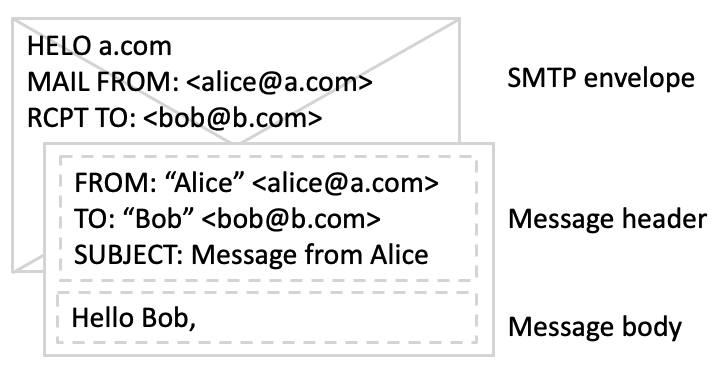
\includegraphics[width=\columnwidth]{fig/mech_smtp_headers.pdf}}
    \centering
    \caption{Example SMTP headers in a transmission (inspired by Figure 3 in Chen et al.~\cite{chen2020composition}).}
    \label{fig:mech_smtp_headers}
\end{figure}

\subsection{Email Spoofing Protections}
The original SMTP design lacks authentication, which
has made email spoofing attacks both possible and common. To mitigate these attacks, the community has proposed multiple mechanisms that focus on authenticating the \emph{domain name} used by the
purported sender.\footnote{True per-sender authentication has long floundered
  due to the lack of effective mechanisms for binding user identities
  with cryptographic credentials at scale.  The best known protocol in
  this space, PGP, has been riddled with security and usability issues
  and remains, at best, a niche protocol.  In this paper, we focus
  exclusively on domain-level sender authentication.} Of these
mechanisms, we focus on SPF~\cite{rfc7208}, DKIM~\cite{rfc6376}, and DMARC~\cite{rfc7489} given their wide adoption.

%\subsubsection{SPF}
\medskip
\noindent\textbf{Sender Policy Framework (SPF)} defines a list of IP addresses permitted to send email on behalf of a domain and a set of actions the recipient should take if they receive an email from an unauthorized IP address.\footnote{In addition to lists of raw IP addresses, SPF
records can also ``include'' other SPF records by reference.}
Domain owners specify this policy by publishing it in a DNS TXT record.
Upon receiving an email message, the receiver fetches the list of authorized sender IP addresses by querying the domain in the email's \textsc{MAIL FROM} header.
The recipient then verifies if the IP address of the sending server is included that list.
If the verification fails, the receiver enforces the action (e.g., marking the email as spam) specified by the \textsc{MAIL FROM} domain in their SPF policy.


% When receiving email from a given IP address, a mail server queries the
% domain present in the \textsc{MAIL FROM} header to obtain its SPF
% policy (encoded in DNS TXT records) and checks whether the policy's list of allowed IP addresses includes the sending server's IP address.
% If the check fails, the mail server then enforces the filtering policy
% specified by the domain owner's SPF policy (\eg, hard fail, soft fail).
% \footnote{Note, it is recommended but not required to also
  % check against the domain identified in SMTP's HELO handshake.}
%
% One major problem with SPF is that it is not compatible with simple
% forwarding. When an email is forwarded, SPF checks can fail because a
% mail server will authenticate the forwarding server, rather than the
% original sending server.

%\subsubsection{DKIM}
\medskip
\noindent\textbf{DomainKeys Identified Mail (DKIM)} cryptographically
binds an email message with its sending email domain.  With DKIM, the
sender signs an email (or certain elements of an email) and attaches a digital signature via a
\textsc{DKIM-Signature} message header for future verification.
Receivers later retrieve the signer's public key (in the form of a DNS TXT record) from the domain specified in the \textsc{DKIM-Signature} header and authenticate an email's signature using that key.

Sadly, neither SPF nor DKIM verify that an email's purported sender (\ie, the \textsc{FROM} header) truly wrote and sent it~\cite{chen2020composition}.
For example, an attacker could bypass DKIM by spoofing an email's \textsc{FROM} header, but then sign and attach a DKIM signature that uses key pairs linked to their own domain (since DKIM does not compare the signature's domain against the \textsc{FROM} domain).
Attacks that exploit
this lack of \textsc{FROM} header authentication motivated the creation of DMARC.
% the \textsc{FROM} header
% displayed to the users, and passing SPF and/or DKIM validation does
% not guarantee the authenticity of the \textsc{FROM} header.  This
% lack, among other reasons, led to the creation of DMARC.

%\subsubsection{DMARC}
\medskip
\noindent\textbf{Domain Message Authentication, Reporting, and
Conformance (DMARC)} combines and extends SPF and DKIM to mitigate these security issues.
% authenticate the domain specified in the \textsc{FROM} header. 
Under DMARC, an email's receiver performs an ``alignment test'': checking if the
domain in the \textsc{FROM} header matches the domain name verified by
either SPF (the domain in the \textsc{MAIL FROM} header) or DKIM (the
domain in the \textsc{DKIM-Signature} header).
By default (``relaxed mode''), the alignment test only requires that the registered domains in the headers match (\ie, not the fully qualified domain name (FQDN)). However, domain owners can specify that recipients should follow the strict mode of the alignment test, which requires the \textsc{FROM} header's FQDN to exactly match the domain authenticated by SPF or DKIM.\footnote{%As with SPF, 
DMARC policy records are also stored as DNS TXT records.} 

If the email passes either SPF or DKIM authentication, and the alignment test also passes, then DMARC considers the email authenticated.
% The alignment test, and overall DMARC authentication for an email, succeeds if 
% The alignment test succeeds if the email passes under either the SPF or DKIM comparison
% When either SPF or DKIM are successful and the alignment test is also successful, the email is considered passing DMARC authentication.
Otherwise, the receiver should implement the DMARC policy designated by the domain in the \textsc{FROM} header, selected from one of three options: \textsc{None},
\textsc{Quarantine}, or \textsc{Reject}.  A policy of \textsc{None}
specifies that an email should be delivered as normal (and thus is often used for monitoring purposes~\cite{DMARCMonitoring1,DMARCMonitoring2}), and \textsc{Reject}
specifies that the recipient mail server should drop the email without
delivering it to the user.  The \textsc{Quarantine} policy is not strictly
defined (indicating only that the message should be treated ``as
suspicious'') and allows each email provider considerable latitude in
their implementation (\eg, setting a UI indicator or placing the email
in a designated spam folder)~\cite{rfc7489}.

%\subsubsection{UI-level Protection}
%% \paragraph{UI Indicators}
%% The combination of these various measures does
%% not always produce a clear binary signal.
%% Thus, email services frequently combine filtering rules with application-layer user interface (UI) indicators to help alert users when the authenticity of an email is suspect.
%% However, currently there is no standard for how and when such
%% UI indicators should be implemented, and different providers favor
%% different approaches.
%% \grant{I think we can completely cut this paragraph if we need space (IV.D.2 gives enough context about UI defenses without this.)}
%% \geoff{looking at IV.D.2, agreed}
% \grant{This part is a little thin, and might be worth folding into the
% vulnerability/attack section where relevant.}\amirian{agreed; it seems out of
% place here. unless this specifically comes into play in the attack section I
% would consider removing it}

% So, in addition to mandatory
% filtering rules, application-layer user interface (UI) indicators are also
% commonly used to help alert users when the authenticity of an email is
% suspect. However, currently there is no standard on how and when such
% UI indicators should be implemented, and different providers favor
% different approaches.

% (1) {\bf
% p=reject} the mail server rejects the email (2) {\bf p=quarantine} the mail
% server accepts the email but marks it as suspicious\gakiwate{Put it in Trash?}
% (3) {\bf p=none} the mail server accepts the email
% nevertheless.\gakiwate{@@Alex: spell out the DMARC policies and expected behavior}

% The DMARC policy None is the weakest and allows for spoofing since an email
% maybe accepted regardless of whether it passes SPF or DKIM. That said, most
% email providers will label such emails as suspicious and display warnings.
% Thus, even though a domain may have DMARC policy None an attacker still may
% have to defeat email providers' protections to deliver an email to the users
% inbox.

% \gakiwate{@@Alex: Make consistent with dmarc policy usage elsewhere.}

% Together these mechanisms can help authenticate emails and thus prevent the
% email spoofing.
%Next, we consider email forwarding and how it complicates these
%email authentication mechanisms.

\begin{figure}[t]
%  \vspace*{-0.2in}
\centerline{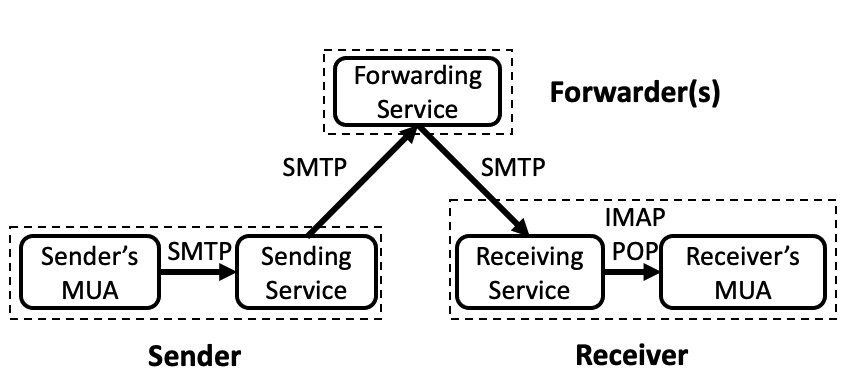
\includegraphics[width=\columnwidth]{fig/mech_email_forwarding_flow.pdf}}
\caption{Email flow involving forwarding.}
\label{fig:email_forwarding_flow}
  \vspace*{-0.1in}
\end{figure}


\subsection{Email Forwarding}
\label{sec:background:fwd:overview}
% \amirian{can you give a one sentence example of a e.g. of a forwarder? someone
% who isnt familiar with forwarders might not understand who can run them and it
% would help to cement the understanding here}
Forwarding is ubiquitous in the email ecosystem and is necessitated by
the wide use of mailing lists~\cite{Electron8:online}, email filtering
services such as ProofPoint~\cite{SecureEm78:online}, and
auto-forwarding employed by individual users for account
aggregation~\cite{TheBestW9:online}, among others.  As shown in
Figure~\ref{fig:email_forwarding_flow}, forwarding alters the standard
transmission flow of an email message.  Instead of a direct
transmission from the sender to the recipient, forwarding relays an
email from the sender to an intermediate server and/or account, which
then transmits a copy of the email to the final recipient.
% (e.g., when a student configures her university email account to forward all messages to a pre-existing personal email address).
For simplicity we show a single forwarder in our example, but email can pass through multiple forwarders in common use cases. % (note, while the figure shows a single forwarder, it is possible to have multiple such forwarders in series).
%While Figure~\ref{fig:email_forwarding_flow}
%shows a single forwarder it is possible to have multiple forwarders.
%Additionally, a forwarder may not always have a domain name associated with it.
%\gakiwate{@@Alex: ProofPoint does not have a domain name no? Check.}

% Forwarders play the same role as receivers but also seek to
% retransmit the original message to a new destination.
Like normal receivers in direct mail transfer,
forwarders are responsible for performing standard authentication checks on each email they receive. % as normally done by a receiver.
However, after authenticating a message,
a forwarder often makes \emph{changes} to the email headers and/or the
email body based on the service it provides.
%(\S~\ref{sec:measure_forwarding_mechs_and_arc}).
The forwarder then sends the modified message to the final receiver (or next forwarder), which also performs authentication checks upon receiving the email.
Finally, when a recipient receives and opens an email, the receiver's user agent (MUA) parses and displays the message to the user.
%If such an email fails DMARC authentication checks at the receiver, the receiver should follow the DMARC policy specified in the email's \texttt{FROM} header.
% Finally, an email is parsed and displayed at the recipient's mail user
% agent.

%. Additionally, most email providers add their own
%warnings if needed based on the email. While an email contains
%multiple headers that represent different sender identities, the MUA
%generally only displays the FROM header and optionally displays other
%headers~\cite{chen2020composition}.
%
% However, the need to accommodate email forwarding while reliably
% authenticating emails introduces challenges. For example, SPF
% validation frequently fails because the receiver will attempt to
% authenticate the forwarding service (which frequently does not have
% the same domain as the \textsc{MAIL FROM} header) rather than the
% original sending server.  Moreover, DKIM checks may fail if a
% forwarder modifies the email body (\eg, many mail filtering services
% rewrite URLs in the email body to offer post-delivery protection). The
% resulting DMARC failures may thus prevent forwarded mail from being
% delivered (\ie, if the \textsc{FROM} domain DMARC policy is quarantine or
% reject).  To prevent this outcome, and preserve the utility of
% forwarders, forwarding services modify email headers to try to ensure
% email delivery. Unfortunately, there is no accepted standard for these
% modifications and different providers use different strategies ---
% \emph{forwarding mechanisms} --- to forward email.  We describe four
% such forwarding mechanisms
% (Figure~\ref{fig:forwarding_mechs_combined}) that are relevant to this
% paper. While some mechanisms are well-documented (\eg, remailing),
% others are ad-hoc and not as well-documented.

%while others are custom and less well-documented \alex{e.g. MAIL FROM equals
%FROM, which is used by outlook}.

% %\subsubsection{Email Forwarding Mechanisms}
% \begin{figure}[t]
%     \centering
%     \includegraphics[width=\columnwidth]{graphs/table_forwarding_mechanisms_combined.png}
%     \caption{Four Types of Forwarding Mechanisms}
%     \label{fig:forwarding_mechs_combined}
% \end{figure}
%
% \noindent{\bf Plain Message-Forwarding (PMF)}. Initially designed for
% the purpose of ``source-routing''~\cite{Emailfor45:online}, PMF was
% one of the first forwarding mechanisms in wide use.  PMF only changes
% the \textsc{RCPT TO} header and leaves other fields
% untouched~\cite{Emailfor45:online} when forwarding.
% Figure~\ref{fig:forwarding_mechs_combined}a depicts the actions of
% such a forwarder which changes the \textsc{RCPT TO} header to the
% address of the receiver (\dns{c@c.com}) and leaves all other fields
% intact.
%
% In general, SPF disallows PMF, since this style of forwarding often
% causes SPF checks to fail at the final receiver.  Nevertheless, as we
% detail later, many email providers, like Yahoo and Fastmail, still use
% PMF in practice, which can result in security issues.
%
% {\bf Remailing (REM)}. Compared to PMF, remailing (aka redistribution),
% works well with SPF. It refers to re-sending a message and also
% rewriting the \textsc{MAIL FROM} field. It is commonly named remailing
% because the process resembles the action of a Mail User Agent
% submitting a new
% message\cite{SenderRe69:online}. Figure~\ref{fig:forwarding_mechs_combined}b
% depicts an example of how headers are modified in remailing. The
% forwarder (\dns{b.com}) first changes the \textsc{RCPT TO} header
% to reflect the destination email address (\dns{c@c.com}). It also
% rewrites the \textsc{MAIL FROM} header to reflect an address in its
% own domain (e.g., \dns{xyz@b.com}).\footnote{The exact username (the
%   ``xyz'' part) in the \textsc{MAIL FROM} address after rewriting
%   depends on the specific implementation.}  The Sender Rewriting
% Scheme, defined in RFC 5231~\cite{rfc5231}, provides a generic
% framework for rewriting email addresses in the \textsc{MAIL FROM}
% header. However, in reality, providers do not strictly follow this
% scheme.
%
% While REM works for well for SPF, it is not very compatible with
% DMARC. Without a valid DKIM header, which can happen sometimes (\eg,
% mailing lists alter a user's post signed by DKIM~\cite{rfc6783}), email
% messages forwarded via REM would fail DMARC's alignment test, and thus
% DMARC authentication. This creates a problem if the \textsc{FROM}
% domain has strict DMARC policies like quarantine or reject.
%
% \noindent{\bf Remailing with Modification (REM + MOD)}. Email
% forwarded by mailing lists that exercise REM and also alter message
% content can also sometimes fail DMARC. Remailing with Modification (REM +
% MOD) was introduced to address this issue and ensures forwarded email
% messages will pass SPF and DMARC. Besides modifying the headers
% mentioned in REM, REM + MOD also rewrites the \textsc{FROM}
% header~\cite{rfc6783}.  Figure~\ref{fig:forwarding_mechs_combined}c
% shows an example of such a modification.  Here, a forwarder
% (\dns{b@b.com}) modifies \textsc{MAIL FROM} and \textsc{RCPT TO}
% headers like REM.  Additionally, it changes the \textsc{FROM} header
% to an email address in its own domain (\dns{b@b.com}).
%
% While fully compatible with DMARC, for the same reason REM + MOD also
% introduces new security concerns. A spoofed email forwarded via REM +
% MOD is ``laundered'' with a new set of headers that will always pass
% SPF and DMARC checks, making it no different than other legitimate
% email messages.
%
%
% \noindent{\bf MAIL FROM Equals From (MFEF)}. Unlike the three
% forwarding mechanisms described above, for which we can find some
% public documentation, MAIL FROM Equals From is a custom forwarding
% mechanism that appears to only be used by Outlook.\footnote{We are not
%   entirely clear what function MFEF serves but we hope, as part of our
%   disclosure interactions with Microsoft, to gain a better
%   understanding of this design's motivation for a future version of
%   this paper.}  An example of MFEF is shown in
% Figure~\ref{fig:forwarding_mechs_combined}d.  In addition to rewriting
% the \textsc{RCPT TO} header to reflect the final receiver
% (\dns{c@c.com}), the forwarder also sets the \textsc{MAIL FROM}
% header to be the same as the \textsc{FROM} header (\dns{a@a.com}),
% regardless of the original \textsc{MAIL FROM} header
% (\dns{z@a.com}). In many scenarios, like PMF, MFEF also will break
% SPF.
%
% %\subsection{Authenticating Email Forwarding}
% %\gakiwate{Can this be confused with simple email forwarding. fwd:
% %  kind?}  As we previously discussed, email authentication using SPF,
% %DKIM and DMARC may lead to email deliverability issues. Thus,
% %forwarders may modify email headers before forwarding to ensure the
% %authentication checks still work.  As such, the receiver implicitly
% %relies on the intermediate forwarders to authenticate the email before
% %modifying it and sending it along.  However, as we demonstrate
% %(Section~\ref{sec:vulnerabilities_in_the_wild}) these assumptions may
% %not always
%
% %For example, an adversary could coax a
% %legitimate forwarder to forward a spoofed email by manually whitelisting domains
% %(Section~\ref{subsec:attack_open_forwarding}). Perhaps more egregiously, some
% %forwarders do not enforce DMARC and forward every email they receive
% %(Section~\ref{subsec:vul:no_dmarc}). Moreover, even the receiver could
% %incorrectly handle the authentication of forwarded emails
%
% \subsection{Authenticated Received Chain}
% \label{sec:arc}
%
% Given the limitations of SPF, DKIM, and DMARC in the presence of
% forwarding, a new mechanism called Authenticated Received Chain
% (ARC)~\cite{rfc8617} was recently introduced to preserve email
% authentication results across multiple forwarders.  ARC chains enable
% a receiver, who might otherwise discard a message, to evaluate the
% full set of intermediary forwarders involved in transmitting the email
% in order to make appropriate exceptions and allow legitimately
% forwarded messages to be delivered~\cite{ARCSpeci1:online}.
%
% %ARC was proposed to solve the deliverability issue introduced by forwarding.
% Intermediary hops implementing ARC sign their authentication results
% (using ARC specific headers) so that these results are accessible by the
% receiver. The expectation is that, in the case where DMARC authentication fails,
% if an ARC chain is present
% %and validated,
% a receiver might choose to
% evaluate the ARC results and allow legitimate emails to be delivered.
%
% However, ARC is currently an experimental standard and only
% implemented by a few providers~\cite{rfc8617, ARCSpeci1:online}. Among
% these, many providers maintain a list of trusted forwarders that
% implement ARC~\cite{Senderau57:online} instead of trusting all
% ARC forwarders. However, any such trust implicitly
% assumes that those trusted forwarders have good security practices.
% Unfortunately, as we detail later, this is not always the case, which
% creates additional opportunities for adversaries
% (Section~\ref{subsec:attack_zoho_arc}).

\subsection{Related Work}

Email security has been a long-standing problem and a variety of prior research efforts have examined different aspects of it. One line of work focuses on understanding and defending against phishing attacks. This includes papers that design new tools for detecting both traditional phishing and sophisticated spearphishing attacks~\cite{abu2007comparison,bergholz2008improved, fette2007learning, garera2007framework, whittaker2010large, duman2016emailprofiler, khonji2011mitigation, zhao2016optimizing, stringhini2015ain, ho19, ho17, cidon19},
study the characteristics of real-world phishing attacks~\cite{han2016phisheye,onaolapo2016happens,thomas2014consequences,bursztein2014handcrafted}, and examine the human aspect of such attacks~\cite{lastdrager2017effective, reinheimer2020investigation,abu2007comparison,
mayer2022don,caputo2013going,
Spero20, Sheng10, Kumaraguru10}.

Another body of work investigates the security and deployment of email encryption mechanisms, such as PGP~\cite{muller2019johnny, poddebniak2018efail, schwenk2020mitigation, muller2020mailto,stransky202227}, DANE~\cite{lee2022under,lee2020longitudinal}, and STARTTLS~\cite{zakir15,Foster15,poddebniak2021tls,holz2015tls,mayer2016no}.

A third research direction analyzes the security and deployment of anti-spoofing protocols such as SPF, DKIM and DMARC, with efforts from both industry and academia. The blogposts by Ullrich~\cite{Breaking12:online} and Haddouche~\cite{Mailsplo10:online} investigated approaches for bypassing DKIM and DMARC using malformed email messages.
Other work has empirically measured the efficacy and deployment status of SPF, DKIM, and DMARC~\cite{hu_end--end_nodate, zakir15, Foster15, tatang2021evolution, deccio21, wang2022large, bennett2022spfail}, as well as qualitatively characterized the factors that drive DMARC policy decisions~\cite{hutowardsunderstanding}.
% systematically researched the deployment of SPF, DKIM and DMARC, including
% the empirical study by Hu \etal\ of anti-spoofing efficacy among
% providers, a subsequent qualitative study
% to investigate the
% factors that
% drive DMARC policy decisions~\cite{hutowardsunderstanding}, and empirical measurement studies of the deployment of SPF, DKIM and DMARC by Durumeric et al.~\cite{zakir15}, Foster et al.~\cite{Foster15}, Tatang et al.~\cite{tatang2021evolution}, Deccio et al.~\cite{deccio21} and Wang et al.~\cite{wang2022large}.

The work most related to our own includes Chen et al.'s analysis of
the security vulnerabilities introduced by protocol composition in
modern email delivery~\cite{chen2020composition}, Shen et al.'s
analysis~\cite{shen2020weak} of modern sender spoofing attacks, and Wang et al.'s~\cite{wang2022revisiting} analysis of email security under the experimental Authenticated Received Chain (ARC) protocol~\cite{rfc8617}.
Of these, Chen et al.~\cite{chen2020composition} do not consider forwarding at all and Wang et al.~\cite{wang2022revisiting} focus on ARC and only consider one specific forwarding implementation as well (REM+MOD in Section~\ref{sec:measure_forwarding_mechs_and_arc}), leaving many other vulnerable forwarding mechanisms and features unexplored.

Shen et al.'s work~\cite{shen2020weak} is the closest in that it also
examines open forwarding, but because they only consider one
forwarding mechanism (what we label as REM in
Section~\ref{sec:measure_forwarding_mechs_and_arc}), they do not
identify the significant scope of this issue.  We build on and
generalize this work to show, among other attacks, that attackers are
able to practically abuse open forwarding to spoof \emph{any} domain
that includes the forwarding domain's SPF record in their own SPF record (a
common practice when hosting email via Microsoft's Outlook service for example).

% and does not illuminate many of the attacks described in our work.
% in Section~\ref{subsec:attack_open_forwarding}

%Additionally, we show how a bug they disclosed in Zoho's ARC implementation, they did not demonstrate how to use this vulnerability in practical attacks.
% due to their limited scope
%In contrast, we present a viable attack that allows an adversary to deliver spoofed email messages addressed from arbitrary domains to arbitrary Zoho users (Section~\ref{subsec:attack_zoho_arc}).
% Similarly, while they were the first to disclose Zoho's buggy ARC implementation, they missed the attack we describe in Section~\ref{subsec:attack_zoho_arc} due to limited scope --- that they only examined ARC in the context of Gmail and Zoho and did not consider forwarding configurations, which are critical components that enable the attack.

In summary, our work builds on the insights of prior efforts, but focuses exclusively and deeply on the particular security challenges introduced by the design and features of common forwarding mechanisms, and their complex interactions with existing email protocols. Through systematic measurements and analysis, we not only show that prior work largely underestimates the risks of open forwarding,
% (Section~\ref{subsec:attack_open_forwarding}),
but also reveal new attacks not discovered in prior work.
%(Section~\ref{sec:attacks}).



%Since
%forwarding is not the main focus of Shen et al.~\cite{shen2020weak},
%they only present a limited set of results: (1) their forwarding
%mechanism is limited to REM, understating many of the potential
%security issues (2) They examine open forwarding in the context of
%REM, (3) they do not elaborate on capacity of attacks introduced by
%certain vulnerabilities (\eg, the Zoho bug). (4) their work is limited
%to mail providers. In comparison, our work: (1) performs a systematic
%and empirical analysis of forwarding mechanisms used in wild,
%discovering three other broad types of forwarding mechanisms (2)
%Comprehensively measures vulnerabilities exist at all parties involved
%in the email forwarding flow \alex{we omit vulnerabilities they
%  discovered but not used in our attacks} (3) Uncovers security issues
%associated with certain vulnerabilities that are understated (\eg,
%open forwarding and Zoho's ARC bug). Our work also leads to a patch of
%the ARC bug by Zoho (\S~\ref{sec:disclosure}). (4) We also consider
%security issues centered around another common use case of forwarding
%--- mailing lists.

%Besides~\cite{shen2020weak}, other work has talked about different
%ways of bypassing email security protocols. For example,

%\alex{Phishing citations cam be added later}



\section{Email Forwarding in Practice}
% \section{The Challenges with Email Forwarding}
\label{sec:measure_forwarding_mechs_and_arc}

Despite the ubiquity of email forwarding, there is no single and
universally agreed-upon method for how email services should implement
forwarding, resulting in several different approaches~\cite{Emailfor34:online}.  This
heterogeneity stems in part from the difficulty of balancing
compatibility with anti-spoofing protocols and the functional goals of
many forwarding use cases: to transparently hide the intermediate
forwarder and present the illusion that the recipient receives the
email directly from its original sender.

Absent a clear standard to depend on, we have used empirical
measurements to \emph{infer} the forwarding behavior deployed by
prominent email providers and mailing list services.  For each
service, we created multiple test accounts, used them to forward email
to recipient accounts we controlled, and then analyzed the resulting
email headers to identify the forwarding mechanism employed.
(Section~\ref{sec:methodology} has a more detailed description of our
methodology.)

We constructed a comprehensive and representative set of forwarding services by building on top of prior literature.
In total, we studied 20 distinct, leading email forwarding services.
We started by collecting all email providers studied in prior literature~\cite{chen2020composition,shen2020weak,hu_end--end_nodate,wang2022revisiting}.
We considered an email provider \emph{out of scope} if it meets any of these four criteria: (a) it is no longer active (e.g., excite.com); (b) it does not accept US customers (e.g., all Chinese providers studied in prior work);  (c) it is not open to public registration (e.g., cock.li); or (d) it does not support forwarding (e.g., Protonmail).
Using these criteria, we identified 23 email providers.
Next, we excluded five email providers that prohibited bulk registration (which prevents us from running large-scale measurements), leaving us with 18 email providers.
We then identified and removed duplicate providers that are operated by the same vendor under different names, leading to a total of 14 distinct email providers.
Finally, we augmented this set of forwarding services by searching for popular email providers that supported forwarding and widely-used mailing list services (a common use case overlooked in prior literature), adding two additional email providers (Mail2World and GoDaddy) and four mailing lists.

Our selection of email forwarding services covers a diverse set of countries and real-world use cases (personal and business email), and represents services used by the general public (used by over 46\% of popular Alexa domains and government domains according to Liu et al.~\cite{liu2021s} ignoring email filtering services).
%\alex{42.7\% considering email filtering}. 
We list all email providers and mailing lists in Table~\ref{tab:forwarding_mechs_in_the_wild}.


Through our measurements, we confirmed the use of three common
approaches that are generally known through public documentation, and
identified a fourth uncommon implementation used by
Microsoft Outlook (hence referred to as Outlook) and Freemail.hu (hence referred to as Freemail).
As summarized in
Figure~\ref{fig:forwarding_mechs_combined}, in each approach the
forwarder modifies the sender and recipient fields in the SMTP
Envelope and Message headers before relaying the email to its
recipient.



% By analyzing public documentation and empirically testing popular email services (\S~\ref{sec:fwd_adoption_measurement}), we identified four major approaches to implementing email forwarding.
% \geoff{is this a ``result'' because Microsoft's implementation has to be experimentally discovered?}\alex{it is technically discovered through experiments}

We now describe each of these approaches in detail using two running
examples of common email forwarding use cases.  In the first case,
Alice has configured her university account (\dns{alice@univ.edu}) to
forward to her primary personal account (\dns{alice@gmail.com}).  When
her university account receives email (\eg, from
\dns{sp@hotcrp.com}), forwarding retransmits it to
\dns{alice@gmail.com} in a way that makes it seem like the email comes
directly from the sender (\dns{sp@hotcrp.com}), rather than from her
university account.  In the second case, Bob sends an email to a
mailing list (\dns{list@univ.edu}), which redistributes (forwards) the
email to the list's members (\eg, \dns{user@univ.edu}).


\begin{figure}[t]
  \centering
%  \vspace*{-0.1in}
    \includegraphics[width=0.7\columnwidth]{fig/table_forwarding_mechanisms_combined.pdf}
    \caption[Four Prevalent Approaches to Email Forwarding]{Four prevalent approaches to email forwarding.  Addresses
      in blue correspond to header values rewritten during the
      forwarding process.
      }
    \label{fig:forwarding_mechs_combined}
\end{figure}


% \grant{In MFEF, is there a reason why the MAILFROM is acm instead of hotcrp? If it's to illustrate a change, I suggest we use noreply@hotcrp.com for the sender MAIL FROM addresses.}\alex{fixed}

% \noindent{\bf Plain Message-Forwarding (PMF)}.
\textbf{Plain Message-Forwarding (PMF)}. Initially designed for
the purpose of ``source-routing''~\cite{Emailfor45:online}, PMF was
one of the first forwarding mechanisms in wide use.
Forwarders that use PMF only change
the \textsc{RCPT TO} header from the forwarder's email account (\dns{alice@univ.edu}) to the final recipient's address (\dns{alice@gmail.com}), and leave all other fields
untouched,
%~\cite{Emailfor45:online},
as illustrated in Figure~\ref{fig:forwarding_mechs_combined}a.
This approach achieves the goal of transparent forwarding.
Changing the \textsc{RCPT TO} header will tell mail servers to send the email to the new address's account, and leaving the \textsc{FROM} header intact will
cause the recipient's email client to display the initial sender (\dns{sp@hotcrp.com}),
rather than presenting \dns{alice@univ.edu} as the sender.
% This approach achieves the goal of transparent forwarding, since the email will appear to come from its initial sender (the \textsc{FROM} header displays the original sender).
% However, it will cause SPF validation to fail in many cases, since the \textsc{MAIL FROM} domain may not list the forwarding server's IP address in its SPF allowlist.


% \noindent{\bf MAIL FROM Equals From (MFEF)}.
\textbf{MAIL FROM Equals FROM (MFEF)}.
Similar to PMF, MFEF (Figure~\ref{fig:forwarding_mechs_combined}b) aims to achieve transparent forwarding by preserving the original sender's identity in the \textsc{FROM} header.
Unlike the other forwarding approaches described in this section, MFEF is a custom forwarding implementation that appears to be used only by Outlook and Freemail.
% \footnote{We are not
%   entirely clear what function MFEF serves but we hope, as part of our
%   disclosure interactions with Microsoft, to gain a better
%   understanding of this design's motivation for a future version of
%   this paper.}
A MFEF forwarder not only rewrites the \textsc{RCPT TO} header to the final recipient (\dns{alice@gmail.com}), but it \emph{also} sets the \textsc{MAIL FROM}
header to be the same as the \textsc{FROM} header (from \dns{noreply@hotcrp.com} to \dns{sp@hotcrp.com}).

Email forwarded using PMF and MFEF often break SPF validation because the \textsc{MAIL FROM} domain typically does not list the forwarding server's IP address in its SPF allowlist;
in our example, \dns{hotcrp.com} does not list the email servers for \dns{univ.edu} in its SPF allowlist.
This incompatibility has hindered the adoption of SPF and DMARC~\cite{hutowardsunderstanding},
leading to provider-specific defenses and new anti-spoofing protocols that we describe in Section~\ref{sec:assumptions}.

%Despite these defenses, we show how attackers can abuse forwarding to nonetheless successfully spoof email from hundreds of thousands of popular domains in
%Section~\ref{sec:attacks}.

% Figure~\ref{fig:forwarding_mechs_combined}a depicts the actions of
% such a forwarder which changes the \textsc{RCPT TO} header to the
% address of the receiver (\dns{c@c.com}) and leaves all other fields
% intact.

% In general, SPF disallows PMF, since this style of forwarding often
% causes SPF checks to fail at the final receiver.  Nevertheless, as we
% detail later, many email providers, like Yahoo and Fastmail, still use
% PMF in practice, which can result in security issues.

% {\bf Remailing (REM)}.
\textbf{Remailing (REM)}. Unlike PMF and MFEF, remailing (aka redistribution)
works well with SPF because this approach alters the headers in a way that resembles the action of the forwarder submitting a new message~\cite{SenderRe69:online}.
% It refers to re-sending a message and also
% rewriting the \textsc{MAIL FROM} field. It is commonly named remailing
% because the process resembles the action of a Mail User Agent
% submitting a new
% message\cite{SenderRe69:online}.
As shown in Figure~\ref{fig:forwarding_mechs_combined}c, the REM
forwarder (\dns{univ.edu}'s mail server) first changes the
\textsc{RCPT TO} header to specify the final recipient (\dns{alice@gmail.com}).
Additionally, the forwarder rewrites the \textsc{MAIL FROM} header so that it
corresponds to an address in the forwarder's own domain (\eg,
\dns{alice-xyz@univ.edu}).\footnote{The Sender Rewriting Scheme
(RFC~5231~\cite{rfc5231})provides a generic framework for how forwarders should
rewrite the \textsc{MAIL FROM} header.  However, email providers do not
strictly follow this scheme and the exact email address after rewriting varies
by implementation.}
% \footnote{The exact username of the \textsc{MAIL FROM} address after
% rewriting varies by the specific implementation.}  The Sender Rewriting
% Scheme, defined in RFC 5231~\cite{rfc5231}, provides a generic
% framework for rewriting email addresses in the \textsc{MAIL FROM}
% header. However, in reality, providers do not strictly follow this
% scheme.

However, even though REM interoperates with SPF, it can still fail DMARC
authentication.  Absent a valid DKIM header, email messages forwarded
via REM will fail DMARC's alignment test because the \textsc{FROM}
domain will not match the SPF-verified \textsc{MAIL FROM}
domain.\footnote{Many domains still do not implement DKIM for outbound email, and even
  those that do can have their user's DKIM signatures invalidated by mailing
  list software that adds content to a user's post~\cite{rfc6783}.}
This incompatibility has led to the common adoption of weaker DMARC policies,
such as \textsc{None} and \textsc{Quarantine} instead of
\textsc{Reject}~\cite{hutowardsunderstanding}.

% This creates a problem if the \textsc{FROM}
% domain has strict DMARC policies like quarantine or reject.

% \noindent{\bf Remailing with Modification (REM + MOD)}.
\textbf{Remailing with Modification (REM + MOD)}.
The final forwarding approach, Remailing with Modification (REM + MOD)~\cite{rfc6783},
resolves these compatibility issues by sacrificing the goal of transparent forwarding.
Email forwarded using REM + MOD will pass both SPF and DMARC.
However, email forwarded with this approach will display the \textit{forwarder} as the email's sender to the final recipient (hiding the identity of the original sender).
Because of this functional change, most major email platforms do not adopt this approach, and it is used primarily by mailing list services such as Gaggle.

As shown in Figure~\ref{fig:forwarding_mechs_combined}d, with REM + MOD the forwarder modifies the headers just like it would during REM forwarding: changing the \textsc{RCPT TO} header to the final recipient (\dns{user@univ.edu}) and the \textsc{MAIL FROM} header to an address in the forwarder's domain.
Additionally, the forwarder rewrites the \textsc{FROM} header to match its account or an email address within its domain (e.g., \dns{list@univ.edu}).

Although this forwarding approach produces email messages compatible with DMARC,
we found that it also introduces a new set of security concerns and spoofing attacks (\S~\ref{subsec:attack_none_mailing_list}).
At a high-level, because REM + MOD rewrites a forwarded email's headers to always pass SPF and DMARC checks, it enables an attacker to launder a spoofed email through a vulnerable forwarder such that it appears like a legitimate email message to the recipient.

% To resolve these compatibility issues with security protocols,
% one forwarding approach, Remailing with Modification (REM + MOD), choses to sacrifice the goal of transparent forwarding to ensure that forwarded emails pass both SPF and DMARC.
%
% As seen in Figure~\ref{fig:forwarding_mechs_combined}c, during REM + MPD, the forwarder modifies the headers just like it would during REM forwarding: changing the recipi
%
% Remailing with Modification (REM + MOD) allows emails to pass both SPF and DMARC, however the emails forwarded under this approach will display the forwarder as the email's sender to the final recipient (hiding the identity of the original sender).
%
% Email forwarded by mailing lists that exercise REM and also alter message
% content can also sometimes fail DMARC. Remailing with Modification (REM +
% MOD) was introduced to address this issue and ensures forwarded email
% messages will pass SPF and DMARC. Besides modifying the headers
% mentioned in REM, REM + MOD also rewrites the \textsc{FROM}
% header~\cite{rfc6783}.
%
% Figure~\ref{fig:forwarding_mechs_combined}c
% shows an example of such a modification.  Here, a forwarder
% (\dns{b@b.com}) modifies \textsc{MAIL FROM} and \textsc{RCPT TO}
% headers like REM.  Additionally, it changes the \textsc{FROM} header
% to an email address in its own domain (\dns{b@b.com}).

% While fully compatible with DMARC, for the same reason REM + MOD also
% introduces new security concerns. A spoofed email forwarded via REM +
% MOD is ``laundered'' with a new set of headers that will always pass
% SPF and DMARC checks, making it no different than other legitimate
% email messages.

% \begin{table}[t]
% \centering
% \begin{tabular}{lll}
% \toprule
% \textbf{Provider} & \textbf{Fwd. Mechanism} & \textbf{ARC} \\
% \midrule
% Gmail         & REM                & \checkmark            \\
% Outlook       & MFEF               & \checkmark            \\
% Zoho      & REM                & \checkmark            \\
% Fastmail      & PMF                & \checkmark            \\
% Yahoo         & PMF                &             \\
% GMX           & REM                &             \\
% Mail.Ru           & PMF                &             \\
% Inbox.lv           & REM                &             \\
% Mail2World.com           & PMF                &             \\
% \midrule
% Google Groups & REM          & \checkmark            \\
% Gaggle  & REM + MOD          &             \\
% Listserv      & REM                &             \\
% Mailman       & REM                & \checkmark \\
% \bottomrule
% \end{tabular}
% \caption{Default forwarding mechanisms and ARC support of the providers and mailing list services we tested.
% \grant{Let's remove the ARC column?}\alex{ok}
%   \label{tab:forwarding_mechs_in_the_wild}}
% \end{table}


%% \begin{table}[t]
%%   \centering
%%   \begin{tabular}{ll}
%%   \toprule
%%   \textbf{Provider} & \textbf{Forwarding Approach}  \\
%%   \midrule
%%   Gmail         & REM                       \\
%%   Outlook       & MFEF                        \\
%%   Zoho      & REM                          \\
%%   Fastmail      & PMF                         \\
%%   Yahoo         & PMF    \\
%%   GMX           & REM    \\
%%   Mail.Ru           & PMF     \\
%%   Inbox.lv           & REM   \\
%%   Mail2World.com           & PMF    \\
%%   \midrule
%%   Google Groups & REM            \\
%%   Gaggle.email  & REM + MOD         \\
%%   Listserv      & REM        \\
%%   Mailman       & REM       \\
%%   \bottomrule
%%   \end{tabular}
%%   \caption{Default forwarding mechanisms and ARC support of the providers and mailing list services we tested.
%%     \grant{The other/alternate version looks great (and uses less room than this)!}
%%     \geoff{I'll experiment with alternate formats}
%%     \label{tab:forwarding_mechs_in_the_wild}}
%%   \end{table}

\begin{table}[t]
  \centering
  \begin{tabular}{ll|ll}
  \toprule
\multicolumn{2}{l}{\textbf{Email} \hfill \hspace*{0.22in}\textbf{Forwarding}} & \textbf{Mailing} & \textbf{Forwarding} \\
\multicolumn{2}{l}{\textbf{Provider} \hfill \hspace*{0.05in}\textbf{Mechanism}} & \textbf{List Service} & \textbf{Mechanism} \\
  \midrule
  Fastmail        & PMF  & Gaggle & REM+MOD \\
  Freemail.hu     & MFEF & Google Groups & REM\\
  GMX/Mail.com    & REM  & Mailman & REM  \\
  Gmail           & REM  & Listserv & REM \\
  GoDaddy         & REM  & & \\
  Hushmail        & PMF  & & \\
  iCloud          & PMF  & & \\
  Inbox.lv        & REM  & & \\
  Mail.ru         & PMF  & & \\
  Mail2World      & PMF  & & \\
  Onet.pl/Op.pl   & REM  & & \\
  Outlook/Hotmail/O365 & MFEF & & \\
  Pobox           & REM  & & \\
  Runbox          & PMF  & & \\
  Yahoo           & PMF  & & \\
  Zoho            & REM  & & \\
  \bottomrule
  \end{tabular}
  \caption[The Providers and Mailing List Services Tested]{The providers and mailing list services we tested and the forwarding mechanisms they use. For providers that are operated by the same vendor under different names (e.g., GMX and Mail.com), we merge them into one row. O365 stands for Office 365.
    \label{tab:forwarding_mechs_in_the_wild}}
  %\vspace*{-0.2in}
  \end{table}

%\subsection{Adoption of Forwarding Approaches}
%\label{sec:fwd_adoption_measurement}

% % We used controlled experiments to evaluate the forwarding behavior of
% % nine prominent email providers
% % and four popular mailing list services.
% We empirically assessed which forwarding strategy different prominent email providers and mailing list servers have adopted.
% %\footnote{
% Our goal was to cover as many providers as possible that are studied
% in prior
% work~\cite{chen2020composition,shen2020weak,hu_end--end_nodate}, while
% filtering out providers that do not support forwarding.  We also skipped
% providers for which we had trouble registering accounts due to
% specific registration requirements (\eg,
% all Chinese providers), for which we could not bypass bot detection
% (\eg, Yandex), and those that make bulk registration challenging (\eg,
% iCloud). Notably, we study Google and Microsoft, which are prominent
% among popular domains according to Liu \etal~\cite{liu2021s}.
% \geoff{the current description is subtractive; another approach
%   is to have it be additive (cover prominent according to Liu +
%   mailing lists), and then describe that there are others we tried
%   for additional coverage but had the issues listed}\alex{I kinda like the additive one. See below}

% \alex{Additive version}

Table~\ref{tab:forwarding_mechs_in_the_wild} summarizes the default forwarding approach used by each of the email providers and mailing lists in our study.\footnote{A provider might forward differently when forwarding between internal accounts, and a mailing list might switch to a different forwarding mechanism to avoid issues caused by forwarding email messages from domains with stricter DMARC policies~\cite{spamreso59:online}. We do not consider these two cases.}
%
% \subsection{Default Forwarding Mechanisms}
% \label{subsubsec:measure_fwding_mech}
%
The most common forwarding approach is remailing forwarding (REM),
used by seven email providers (GMX, Gmail, GoDaddy, Inbox, Onet, Pobox, and Zoho) and
three mailing lists (Google Groups, Listserv, and Mailman). Seven email providers, Fastmail, Hushmail, iCloud, Mail.ru, Mail2World, Runbox, and Yahoo, use
plain-message forwarding (PMF).
% while
Outlook and Freemail use their own custom
forwarding mechanism (MFEF) and, as described, Gaggle uses remailing with modification (REM+MOD)
forwarding.
% \geoff{would ``Gaggle Mail'' be more consistent with how we name providers?}
% described in Section~\ref{sec:background:fwdingmechanisms}.


%\input{3.indi_vulnerabilities.tex}

%% \begin{table*}[t]
%%     \centering
%%     \begin{tabular}{p{17em}p{14em}p{14em}}
%%         \toprule
%%     \textbf{Assumption or Feature}                          & \textbf{Associated Implementation}  & \textbf{Prevalence}    \\
%%     \midrule
%%     Domain will use actionable DMARC policies   & DMARC none & Two thirdsSecurity of popular Alexa domains that have DMARC \\
%%     %\hline
%%     Each domain uses its own infrastructure  & Shared SPF record    & All providers \alex{Fastmail? Forwarding infra?}  \\
%%     Quarantining an email neutralizes its threat    & Quarantine instead of reject    & Outlook, Fastmail, GMX and Inbox.lv \\
%%     Allowing users to override DMARC decisions    & Domain whitelisting    & All providers  \\
%%     %\hline

%%     Users only forward to accounts they control   & Open forwarding    & Outlook, Fastmail and Mail2world.com \\
%%     Forwarded email from large providers are likely benign  & Relaxed validation & Gmail, Outlook and Mail.ru   \\
%%     %    & Overtrust other providers    & Gmail    \\
%%     %    & ARC bug    & Zoho    \\
%%     %    & UI bug & Gmail \\
%%     Every email is legitimate & Not enforcing DMARC & Gaggle.email and Mail2world.com\\
%%     \bottomrule
%%     \end{tabular}
%%     \captionof{table}{Summary of vulnerable designs and assumptions that attackers can exploit with forwarding.}
%%     \label{tab:assumptions_and_prevalence}
%%     \end{table*}

\begin{table*}[t]
    \centering
    \small
%    \begin{tabular}{lp{17em}p{14em}p{14em}}
    \begin{tabular}{p{0.08\textwidth}p{0.32\textwidth}p{0.3\textwidth}p{0.18\textwidth}}
        \toprule
&     \textbf{Security Assumption or Feature} & \textbf{Implementation Aspect}  & \textbf{Prevalence}    \\
    \midrule
    \S~\ref{subsubsec:dmarc_none} &    Domain will use actionable DMARC policies   & DMARC None & Two-thirds of Alexa Top 1M\\
% Two-thirds of popular Alexa domains using DMARC
    %\hline
    \S~\ref{subsubsec:spf_incorporation} &  Each domain uses its own infrastructure  & Shared SPF record    & All providers \\
    \S~\ref{subsubsec:quarantine_instead_of_reject}    & Quarantining is sufficient    & Quarantine instead of reject    & Outlook, Fastmail, GMX, Inbox.lv, Pobox \\
    \S~\ref{subsubsec:whitelist}    & Per-user DMARC overrides are fate-sharing    & Domain whitelisting    & All providers  \\ [0.15in]
    %\hline

    \S~\ref{subsubsec:open_forwarding}    & Users only forward to accounts they control   & Open forwarding    & Ten providers including Outlook and Fastmail\\
    \S~\ref{subsubsec:relaxed_validation}    & Forwarded email from large providers benign  & Relaxed validation & Gmail, Outlook, Mail.ru   \\
    \S~\ref{subsubsec:unsolicited_dkim}    & Adding DKIM signature increases deliverability & Unsolicited DKIM signatures & iCloud, Runbox,  Hushmail\\


    %    & Overtrust other providers    & Gmail    \\
    %    & ARC bug    & Zoho    \\
    %    & UI bug & Gmail \\
%    & Every email is legitimate & Not enforcing DMARC & Gaggle.email and Mail2world.com\\
    \bottomrule
    \end{tabular}
    \captionof{table}{Summary of vulnerable security assumptions and forwarding features, the aspect of their implementation that leads to the vulnerability, and the prevalence of the vulnerability.
    }
    \label{tab:assumptions_and_prevalence}
%    \vspace*{-0.2in}
    \end{table*}

% \section{Assumptions Violations and Implementation Errors in Practice}
% \section{Vulnerable Security Assumptions and Forwarding Mechanisms}
% \section{Vulnerabilities, Assumptions and Bugs}
\section{Assumptions and Vulnerable Features}
\label{sec:assumptions}

In this section, we describe a range of email design and
implementation weaknesses that lead to forwarding vulnerabilities.
We start by exploring four assumptions made by anti-spoofing mechanisms
that email forwarding can bypass and violate.  We then examine
three vulnerable forwarding features in the major forwarding
approaches.

%Finally, we also identify
%three
%implementation
%vulnerabilities that are less fundamental, but can still lead to email
%spoofing via forwarding.
In each of these cases, we use active
measurements --- either of mail services themselves or the DMARC policies
as stored in DNS --- to document the prevalence of each issue
among prominent domains and
providers (summarized in Table~\ref{tab:assumptions_and_prevalence}).
In the remainder of this section, we discuss the measurement
methodology used to investigate and identify these issues and
describe each vulnerability in turn.  In the next section,
% (Section~\ref{sec:attacks})
we then show how these vulnerabilities can
be combined to create complete and effective spoofing attacks
involving a broad array of popular and sensitive domains.

% header rewriting performed during forwarding and vulnerabilities across these two categories to launch attacks that can successfully spoof email from thousands of prominent domains, such \dns{state.gov} and \dns{hulu.com}.

% Additionally, we discuss three implementation vulnerabilities that enable a few novel attacks in Section~\ref{sec:attacks}, which we uncovered during the course of our experiments.



% In this section we examine a set of vulnerable assumptions and implementations across popular email providers and anti-spoofing mechanisms,
% and preview how an attacker can use email forwarding to violate and exploit these design decisions.
% Table~\ref{tab:assumptions_and_prevalence} summarizes our findings, as well as the prevalence of each vulnerability across the email ecosystem.

\subsection{Methodology}
\label{sec:methodology}

%% \geoff{how much of this part of the methodology overlaps with
%%   the methodology described in III.B?
%%   if it is the same, then we can just refer back to III.B}\alex{III.B is rather simple. This seems to be a more detailed version of what's in III.B}
%%   \grant{The first sentence above has some repetition, but I think the rest might be distinct?}\alex{note from the discussion Geoff and I had: We don't run seperate experiments for section 3 and 4, so it might be less confusing if we describe everything here and forward reference in sec 3. Also todo@Geoff, revisit our experiments details and see if anything needs to be added back}

For our experiments we created test \textit{forwarding} accounts on all 20 forwarding services,
test \textit{recipient} accounts on all 16 major
email providers, and mail servers for domains we control as
the \textit{sending} accounts.
%
%% For the email providers, we created test accounts on each platform and
%% configured them to forward email to accounts we controlled.
%% We created mailing lists using each of the services and performed a
%% similar analysis that collected the headers of email we sent to each
%% list.
%
For Google Groups and Gaggle, we created mailing lists under our
university's existing service and at \dns{gaggle.email}, respectively.
The other two mailing list services (Listserv and Mailman) rely upon a
third-party backend mail server; we used
Postfix~\cite{ThePostf34:online} as the backend with DMARC
enforced. We then created mailing lists under new domains we acquired
for testing (\eg, \dns{list@listserv.ourdomain.com}).

%% We recorded the resulting headers at both the forwarder and the final
%% recipients for analysis.

For each combination of forwarding and recipient accounts, we sent
email using three different control domains in the FROM headers, each
with the same SPF configuration but with distinct DMARC policies:
\textsc{None}, \textsc{Quarantine}, and \textsc{Reject}.
%
Some services (\eg, Gmail and Outlook) will mark email messages sent
from new domains as spam until there is sufficient user interaction
with those messages.  To avoid this startup effect, we ``warmed up''
our domains using a series of legitimate exchanges.  In particular,
from each domain, we sent legitimate (\ie, unspoofed) email that
passed SPF, DKIM and DMARC to our accounts at each provider.  Any
message that was delivered to the spam folder we manually marked as
``not spam''.  After this warm up period, we validated that legitimate
(\ie, unspoofed) email from our domains was properly delivered to
account inboxes in all cases.
% for all email providers.

Having primed our accounts, we assessed the prevalence of each vulnerability by
% ran a series of experiments that
sending legitimate and spoofed email messages to all
pairwise combinations of our forwarding and recipient accounts.\footnote{Our code for automatically sending these messages is available upon request.}  We
analyzed the headers and outcomes of these attempts, and recorded
which parties exhibited vulnerable behavior.  In particular, we
configured all forwarders to forward email messages to all receivers
and recorded whether each message was delivered to the inbox, spam
folder, or rejected without delivery by each receiver.  We also noted
whether any UI warning was shown in the native web-based MUA. 


% email ecosystem.


%% \geoff{did we also do
%%   some warm up to establish baseline benign conversations?}\alex{we
%%   did, but I think we removed that part intentionally to avoid any
%%   confusion. We can add them back}

% We start with a set of three new domains under our control.  We
% configure all three with the same SPF configuration, while each of the
% individual domains have a DMARC policy none, quarantine, and reject,
% respectively.  We use these domains in the FROM headers in all of our
% email messages, so that our measurements do not affect users of any
% other domains.

% We then ``warm up'' our domains so that they are treated like any
% other domains by the providers. This ``warm up'' phase is necessary as some providers (e.g., Gmail) would quarantine email messages from a domain if it has never seen an email from that domain before. We ``warm up'' our domain by sending legitimate email messages
% from these domains that pass SPF, DKIM and DMARC to accounts under our
% control at each email provider.  We also manually mark our email
% messages as ``not spam'' if they are delivered to the spam folder in
% the warm-up stage.  After the warm-up stage, legitimate email messages
% from our domains are properly delivered to account inboxes for all email providers.

% We then send legitimate and spoofed email messages from our domains to
% forwarding accounts and record whether a message is forwarded by
% default.  We consider all nine providers and four mailing lists as
% forwarders.  We send spoofed email messages from a server we own that
% is not allowed in the SPF records of our domains.

% We study each receiver's behavior for both legitimate and spoofed
% forwarded email messages. We only consider the nine mail providers as
% receivers, as mailing lists are rarely the destination of email. We
% configure all forwarders to forward email messages to all receivers
% and record whether each message is delivered to the inbox, spam
% folder, or rejected without delivery by each receiver. We also note
% whether any UI warning indicator is displayed in the native web-based
% MUA.

% We force the forwarding of a spoofed email by manually whitelisting it
% at the forwarder. Whitelisting spoofed email messages could be done at
% most forwarders with a few exceptions. We are not able to whitelist
% spoofed email messages at Yahoo in cases where the spoofed FROM domain
% has DMARC policies quarantine or reject. Additionally, we cannot
% whitelist spoofed email messages at Google, Mail.ru and Zoho when the spoofed FROM domain has DMARC policy reject.

% We ensure that our measurement results are reliable by repeating the
% above process with another set of three domains and fresh email
% accounts. We are also aware that all mail providers we study have
% implemented anti-spam systems, which could interfere with our
% measurement results. To minimize the interference from those systems,
% we only send email messages with legitimate content. In cases where we
% observe an inconsistency in a provider's behavior between multiple
% trials (potentially due to triggering the anti-spam system), we
% perform additional measurements with fresh accounts.



% Subsequently, in Section~\ref{sec:attacks}, we show how attackers can combine
% email forwarding with several vulnerabilities to launch successful attacks, allowing them to reliably spoof email from thousands of prominent domains, such \dns{state.gov} and \dns{hulu.com}.
% that email providers and security mechanisms make and
% how forwarding allows an attacker to violate each assumption.
% Additionally, for each vulnerability, we measured and report which email services are impacted.
% In Section~\ref{subsec:assumptions}, we examine a list of assumptions and why they can cause security concerns. Further, to understand whether these security concerns are real, we perform controlled experiments that allow us to observe implementation decisions made by each party that are related to these assumptions.

%%%%%%%%%%%%%%%%%%%%%%%%%%%%%%%%%%%%%%%%%%%%%%%%%%%%%%%%%%%%%%%%%%%%%%%%%

% We start by sending legitimate and spoofed email messages from domains we control to all forwarders. We consider all nine providers and four mailing list services as forwarders. Next, we try forwarding email messages from all forwarders to all receivers. We only consider the nine mail providers as receivers, as mailing lists are rarely the destination of an email. We note and record implementation decisions made by each party that are related to the assumptions we listed.
%
% We ensure that our measurement results are reliable by doing the above measurement twice with two distinct sets of domains that we control. We are also aware that all mail providers we study have
% implemented anti-spam systems, which could interfere with our
% measurement results. To minimize the interference from those systems,
% we only send email messages with legitimate content. In cases where we
% observe an inconsistency in a provider's behavior between multiple trials (potentially due to triggering the anti-spam system), we perform additional measurements with fresh accounts.


% Table~\ref{tab:assumptions_and_prevalence} lists our results. \alex{I should elaborate?}. In the process of doing our measurement, we further observe two implementation errors made by Gmail and Zoho, which we detail in Section~\ref{subsec:implementation_errors}.

%%%%%%%%%%%%%%%%%%%%%%%%%%%%%%%%%%%%%%%%%%%%%%%%%%%%%%%%%%%%%%%%%%%%%%%%%

% We start with a set of three new domains under our control.  We
% configure all three with the same SPF configuration, while each of the
% individual domains have a DMARC policy none, quarantine, and reject,
% respectively.  We use these domains in the FROM headers in all of our
% email messages, so that our measurements do not affect users of any
% other domains.

% We then ``warm up'' our domains so that they are treated like any
% other domains by the providers. This ``warm up'' phase is necessary as some providers (e.g., Gmail) would quarantine email messages from a domain if it has never seen an email from that domain before. We ``warm up'' our domain by sending legitimate email messages
% from these domains that pass SPF, DKIM and DMARC to accounts under our
% control at each email provider.  We also manually mark our email
% messages as ``not spam'' if they are delivered to the spam folder in
% the warm-up stage.  After the warm-up stage, legitimate email messages
% from our domains are properly delivered to account inboxes for all email providers.

% We then send legitimate and spoofed email messages from our domains to
% forwarding accounts and record whether a message is forwarded by
% default.  We consider all nine providers and four mailing lists as
% forwarders.  We send spoofed email messages from a server we own that
% is not allowed in the SPF records of our domains.

% We study each receiver's behavior for both legitimate and spoofed
% forwarded email messages. We only consider the nine mail providers as
% receivers, as mailing lists are rarely the destination of email. We
% configure all forwarders to forward email messages to all receivers
% and record whether each message is delivered to the inbox, spam
% folder, or rejected without delivery by each receiver. We also note
% whether any UI warning indicator is displayed in the native web-based
% MUA.

% We force the forwarding of a spoofed email by manually whitelisting it

% at the forwarder. Whitelisting spoofed email messages could be done at
% most forwarders with a few exceptions. We are not able to whitelist
% spoofed email messages at Yahoo in cases where the spoofed FROM domain
% has DMARC policies quarantine or reject. Additionally, we cannot
% whitelist spoofed email messages at Google, Mail.ru and Zoho when the spoofed FROM domain has DMARC policy reject.

% We ensure that our measurement results are reliable by repeating the
% above process with another set of three domains and fresh email
% accounts. We are also aware that all mail providers we study have
% implemented anti-spam systems, which could interfere with our
% measurement results. To minimize the interference from those systems,
% we only send email messages with legitimate content. In cases where we
% observe an inconsistency in a provider's behavior between multiple
% trials (potentially due to triggering the anti-spam system), we
% perform additional measurements with fresh accounts.




% For assumptions made by senders, we use results reported in prior work~\cite{tatang2021evolution}. For assumptions made by forwarders and receivers, we perform our own measurements as detailed in Section~\ref{subsec:measure_assumptions}.


% \subsection{Assumptions Made in Practice}
\subsection{Email Security Assumptions}
\label{subsec:assumptions}
Anti-spoofing mechanisms define a set of validation procedures which
both explicitly and implicitly rely on assumptions about the behavior
of domain holders, email providers and users.  Here we identify four
such assumptions that are crucial to these defenses in the direct
single-hop delivery context, but do not necessarily hold in the
presence of email forwarding.

% communication,


% In this subsection, we explore different design decisions and assumptions made by email protocols and providers, why forwarding makes them vulnerable to attacks, real-world implementations associated with each vulnerable design.
% Here, we focus on vulnerabilities that are difficult to fix without altering standard email practices or requiring additional action from users and organizations.
% cover harder-to-fix assumptions, why they can be problematic, and real-world implementations associated with each assumption.

\subsubsection{Domains use actionable DMARC policies}
\label{subsubsec:dmarc_none}
DMARC enables recipients to authenticate whether an email truly
originates from its purported sending domain.  However, when a
recipient encounters a spoofed or illegitimate email that fails
authentication, DMARC relies on the true domain owner to specify a
policy for how to treat such email.  This design assumes that domain
owners will use DMARC policies that result in protective
actions, such as \textsc{Quarantine} or \textsc{Reject}.  When a
domain owner chooses a weaker policy, mail providers deliver the
illegitimate email to a user's inbox even if the DMARC authentication
fails, in accordance with email standards (RFC 7489~\cite{rfc7489}).
Unfortunately, prior work has shown that a large number of domains use
weak DMARC policies of
\textsc{None}~\cite{hu_end--end_nodate,tatang2021evolution,hutowardsunderstanding,
  secplaintxt, maroofi2020defensive, adoptionofschemes}, with roughly
two-thirds of the Alexa Top 1M domains employing such a policy (as of
May 2020).  While poor security hygiene accounts for some of this
outcome, many domains choose a weak DMARC enforcement policy for
deliverability concerns due to incompatibility with forwarding~\cite{hutowardsunderstanding}.

% DMARC allows domain owners to specify how to authenticate emails purporting to come from their domain and to instruct mail providers on how to treat illegitimate and spoofed emails. This implicitly assumes that domains will employ good security practices by setting their DMARC policy to quarantine or reject.  Unfortunately, this policy often leaves recipients vulnerable to spoofing attacks in practice, since most providers deliver email to a user's inbox even if it fails DMARC's authentication checks;
% indeed, this behavior matches the expected behavior defined in RFC 7489~\cite{rfc7489}. While some of the domains certainly have bad security hygienes, others do this for deliverability concerns~\cite{hutowardsunderstanding}.
%
% \alex{We did not measure the number of domains w/ DMARC none ourself.}
% Unfortunately, prior work~\cite{hu_end--end_nodate,tatang2021evolution} has shown that a large number of domains use weak DMARC policies of \textsc{None}. For example, according to Tatang et al.~\cite{tatang2021evolution}, among the Alexa top domains that have DMARC configured, roughly two thirds of them have DMARC policy none (as of May 2020).

% DMARC none is no new face to the security community, and there exists a large body of literature around it~\cite{hu_end--end_nodate, hutowardsunderstanding,
% secplaintxt, maroofi2020defensive, adoptionofschemes}.
Cognizant of this reality, several major email providers have decided to take two types of security actions against email that fails DMARC authentication, regardless of the domain owner's specified policy.
First, as noted in prior work~\cite{hu_end--end_nodate} and confirmed in our own experiments, Outlook quarantines email if it fails DMARC authentication, even when the email's \textsc{FROM} domain has a weak DMARC policy of \textsc{None}.
Second, although Gmail, Onet, and Zoho deliver email that fails DMARC authentication to user inboxes, they will display a UI warning to users who read such messages.

These defenses provide protection against attackers who directly send spoofed email to their victims.  However, as we will show,
%~\ref{subsec:attack_relaxed_forwarding_validation} and~\ref{subsec:attack_none_mailing_list},
email forwarding introduces new complexity that enables attackers to bypass these ad hoc defenses, and thus leverage weak DMARC policies to successfully spoofed email from prominent domains.

% In our experiments we observed two defenses that limit the scope of
% this vulnerability for particular providers. First, as also noted by Hu \etal~\cite{hu_end--end_nodate}, if an email message is
% directly sent to Outlook from our server, Outlook always quarantines it if it fails DMARC,
% regardless of the DMARC policy of the \textsc{FROM} domain. Second, as with other providers Gmail
% and Zoho deliver such email messages to the inbox, but also displaying a UI
% warning to users when they read the message. However, as we detail later in Section~\ref{subsubsec:ui_bug}, deferring this to another component (in this case UI) implicitly assumes the UI warning component functions properly, which is not true for Gmail.
%
%
% Sadly, as we detail later, the protection mechanisms mentioned above do not apply to certain forwarded email messages, allowing an
% adversary to bypass them and deliver spoofed messages
% (Section~\ref{subsec:attack_relaxed_forwarding_validation}). We also demonstrate that when combined with certain forwarding mechanism, an adversary can launder their spoofed email messages from domains with DMARC none through mailing lists such that they look no different than legitimate ones after being forwarded (Section~\ref{subsec:attack_none_mailing_list}).


\subsubsection{Each domain uses its own infrastructure}
\label{subsubsec:spf_incorporation}
The SPF protocol predates the emergence of large third-party email providers.
As a result, SPF implicitly assumes that each organization (domain) maintains its own mailing infrastructure: that the set of authentic server IP addresses specified by a domain's SPF record is not also used by other domains or external users to send email.
Unfortunately, as documented by Liu \etal~\cite{liu2021s} and Holzbauer \etal~\cite{holzbauer2022not}, this assumption is invalid today as many organizations outsource their email infrastructure to the \emph{same} third-party providers such as Outlook and Gmail.  Hence, all of these domains have delegated the right to send on their behalf to the same third-party --- trusting that they will ensure isolation in spite of this blanket authorization.
%These large providers often share the same email infrastructure across all cust%omers (both business and personal accounts), violating the assumptions made by %SPF.

% Back when SPF was first proposed, third-party providers were not common. SPF assumes each domain maintains its own infrastructure. However, the rise of third-party providers has challenged this assumption. As documented by Liu et al~\cite{liu2021s}, third-party providers now play a dominant role in mail service provisioning. Instead having dedicated infrastructure for each customer, these third-party providers often share the same infrastructure across all customers, business or personal. However, this implementation breaks the assumption made by SPF and introduces the potential issue of email spoofing --- an adversary, who controls a personal account with the provider, can spoof as others who share the same infrastructure.

Concretely, our measurements show that all 16 email providers in our study appear to configure their email infrastructure in this shared fashion.
%\alex{VERIFY THIS IS TRUE. how do we even measure this?} \geoff{I added hedge wording}.
Additionally, at least for email messages forwarded in our experiments, all providers but one (Fastmail) use the same set of servers to send both direct email and forwarded email.
%~\alex{VERIFY}.  \geoff{we can say that it is true to the extent of the messages we sent...do any providers happen to mention this in their SPF instructions?}\alex{Updated the text a bit. I don't recall seeing any provider mentioning IPs used for forwarding.}

Since SPF no longer provides isolation in this model, the email
providers in our study effectively \emph{simulate} it by preventing users
from setting arbitrary values in their \textsc{FROM} header.  Thus,
even though each mail provider is empowered to send any email on
behalf of all their mail customers, they prevent customers from taking
advantage of this situation by \emph{internally} restricting the \textsc{FROM} headers of outbound email messages coming from a customer's domain.
%a given domain which mitigates the ability for an attacker to use
%these platforms to directly send spoofed email.
% to users.
While this defense is effective in the absence of forwarding, we will
show how open forwarding mechanisms bypass this filtering (by generating spoofed \textsc{FROM} headers from an \emph{external} server controlled by the adversary),
exposing the latent conflict between SPF's design and modern mail service
use---ultimately allowing unrestricted email spoofing.

%Unfortunately, as we show later in Section~\ref{subsec:attack_open_forwarding},
%attackers can overcome these mitigations by employing forwarding to conduct successful spoofing attacks.


\subsubsection{Quarantining is sufficient}
\label{subsubsec:quarantine_instead_of_reject}
RFC 7489~\cite{rfc5231} suggests that if an email message falls under the scope of a DMARC reject policy, then the receiving server should reject and drop it entirely. However, some providers deviate from this advice by marking it as spam and delivering it to a spam folder, assuming that quarantining a malicious email neutralizes its threat.
Our experiments found that five email providers (Outlook, Fastmail, GMX, Inbox.lv and Pobox) adopt this approach.
% believe that quarantining an email neutralizes its threat and still deliver these messages while labeling them as spam.
Figure~\ref{fig:example_ms_not_rejecting} displays an email message from our tests that shows this behavior: it fails DMARC validation, comes from a domain (\dns{state.gov}) that has a DMARC policy of \textsc{Reject}, but is nonetheless delivered
as ``spam''.

\begin{figure}[t]
    \centering
{
    \setlength{\fboxsep}{0pt}
    \setlength{\fboxrule}{0.5pt}
    \fbox{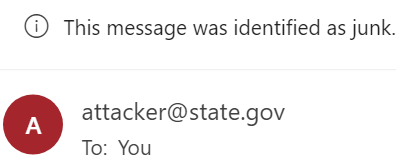
\includegraphics[clip,width=\columnwidth]{fig/ss_outlook_not_rejecting.png}}
}
    %\caption{Example message that has a spoofed FROM header using a domain with DMARC policy reject.  It is delivered to an Outlook user's spam folder instead of being rejected.}
    \vspace*{-0.2in}
    \caption{Example message with a FROM header spoofing a domain with DMARC policy \textsc{Reject}.  Outlook delivers it to the spam folder instead of rejecting it.
    }
    \label{fig:example_ms_not_rejecting}
    \end{figure}

%
% In our experiments, we find that four email providers (Outlook, Fastmail, GMX and Inbox.lv) follow this quarantine-over-reject approach.

Because these providers quarantine the spoofed email as spam, this
design does not appear particularly dangerous.\footnote{Some in the
  mail security industry criticize this weakening of DMARC
  rules and document attacks that ``rescue'' such email from the spam folder via social engineering~\cite{Microsof7:online,Spearphi83:online}.} However, as we
will show, in combination with email forwarding and another
vulnerable feature (per-user domain whitelists in Section~\ref{subsubsec:whitelist}), attackers can override this
protection and exploit the quarantine-over-reject implementation to spoof
email from thousands of popular domains despite their strict
DMARC \textsc{Reject} policy.

%In our work, we present new attacks that show how forwarding introduces a new avenue for exploiting this design.
%In particular, when combined with other vulnerable assumptions (e.g., Section~\ref{subsubsec:whitelist}), attackers can use forwarding accounts to override these quarantine protections and exploit the header rewriting changes in different forwarding approaches to spoof email messages from thousands of popular domains.
%Because of this quarantine-over-reject policy, these attacks are successful even when the spoofed domains have a strict DMARC policy of \textsc{Reject}.

% , and the resulting emails pass both SPF and DMARC validation at the recipient's mail server.

% there have been attacks that explotied this implementation decision as reported in prior blog posts~\cite{Microsof7:online,Spearphi83:online}.
%
% Even worse, as we detail below in Section~\ref{subsubsec:whitelist}, the quarantine decision can be overridden by a malicious user and thus creates a new threat to the downstream providers, potentially allowing an adversary to forward spoofed email messages even if the spoofed FROM domain has DMARC policy reject, endangering downstream providers. Indeed,
% we show in Section~\ref{subsec:attack_open_forwarding} that when an adversary combines such policies with email forwarding and other issues described in this section, they can often spoof email messages from a wide range of domains (even if these domains have DMARC policy reject) that correctly pass both SPF and DMARC validation at the recipient's mail server.

\subsubsection{Per-user DMARC overrides are fate-sharing}
\label{subsubsec:whitelist}
Many email providers allow users to override DMARC decisions: users can whitelist domains, and as a result they will still deliver or forward email even if it fails DMARC.
% \geoff{by ``upon a user's request'', do we just mean that users can whitelist domains to override DMARC?}\alex{yes, updated the text.}
Providers offer this flexibility because it can help mitigate
errors and improve mail deliverability for the users who need it.
However, this feature implicitly assumes that this approach is
fate-sharing --- that when a user overrides DMARC decisions, the risks
of that choice are localized to the individual user account.  While
true in the single-hop context, forwarding again undermines this
assumption.  If adversaries can override DMARC decisions on a
forwarding account they control, they can use that capability to
launder spoofed mail and successfully deliver it downstream.

 % While this can be convenient in certain use cases (e.g., to increase deliverability), it also allows an adversary to potentially forward spoofed email messages. When combined with \emph{open forwarding}, whitelisting enables an adversary to forward spoofed email messages to arbitrary destination, hurting the users of downstream providers and also invalidating the assumption that quarantining an email neutralizes the threat (Section~\ref{subsubsec:quarantine_instead_of_reject}) by introducing a new threat to downstream providers.

Based on our measurements, all mail providers support this functionality in some form.
Of particular note, four of the five providers 
mentioned in Section~\ref{subsubsec:quarantine_instead_of_reject}
(Fastmail, GMX, Inbox.lv, and Pobox)
allow users to override any DMARC decision for any domains.
The fifth (Outlook) allows users to override DMARC decisions for most domains, except for a small set of frequently-spoofed domains that have DMARC policy reject (e.g., \dns{aa.com}) where Outlook appears to apply additional, special protection mechanisms.

% We do not try to whitelist spoofed email messages at mailing list services as generally an adversary cannot have access to a mailing list's configuration. Mail2World.com does not enforce DMARC, so there is no need to override the decision. For the four providers mentioned in Section~\ref{subsubsec:quarantine_instead_of_reject} that do not reject any email, we can override DMARC decisions for all domains for three of them (Fastmail, GMX and Inbox.lv). We are able to override DMARC decision for most domains for Outlook, except for a small set of frequently-spoofed domains that have DMARC policy reject (e.g., \dns{aa.com}). We suspect Outlook has special protection mechanism for these domains.
For Gmail, Hushmail, iCloud, Mail.ru, Onet, and Zoho, users can override DMARC decisions for domains with DMARC policy \textsc{None} or \textsc{Quarantine}, but not \textsc{Reject}.  Finally, for Yahoo, we can only override DMARC decisions for domains with a policy of \textsc{None}.

% but place them in the spam folder instead of the inbox

 % should be rejected but instead delivered to spam.
% The spoofed FROM domain in this case is microsoft.com, which has DMARC policy reject.

% While this vulnerability does not seem to create huge security concerns, there has been reported attacks that exploited such vulnerability.



% Additionally, this vulnerability gives an adversary the ability to whitelist email messages that spoofed from domains with DAMRC reject. As can be seen from Section~\ref{subsec:attack_open_forwarding} and~\ref{subsec:attack_zoho_arc}, combining with other vulnerabilities, this enables an adversary to spoof from arbitrary domains.


 % simply preventing arbitrary FROM header forgery is not enough. A sophisticated adversary, who controls a personal account with third-party providers like Outlook, cam still abuse this shared infrastructure with the help of forwarding.


% \subsection{Assumptions Made in Practice}
\subsection{Vulnerable Forwarding Features}
\label{subsec:fwding_vuln}
In the absence of forwarding, the assumptions described above are
largely benign and allow the effective blocking of many spoofing
attacks.  However, when combined with three vulnerable forwarding
features, open forwarding, relaxed validation, and unsolicited DKIM signatures, the weaknesses in
these assumptions permit several opportunities for bypassing DMARC's
protections.

% and policies
%adopted by major email services that

%, when combined with the header rewriting during forwarding, enable attackers to violate and exploit the security assumptions discussed above.
% \grant{If we go with this structure, we'll need to think about how to word Table~\ref{tab:assumptions_and_prevalence}, or how to reword the vulnerable forwarding features/designs in this subsection.}

% \subsubsection{Users only forward to accounts they control}
% \subsubsection{Forwarding occurs benignly between accounts}
\subsubsection{Open Forwarding}
\label{subsubsec:open_forwarding}
% \alex{Open forwarding}
Many email service providers support a mechanism to automatically
forward a user's messages to another account (\eg, to aggregate mail
sent to multiple addresses into a single inbox).  Because of the
prevalence of these common, benign forwarding use cases, many
platforms follow a design that we call \emph{open forwarding} (also
referred to as ``unauthorized forwarding'' in previous work~\cite{shen2020weak}).  Services with open forwarding allow users
to configure their account to forward messages to any destination
email address, \textit{without} any verification from the destination
address.  Open forwarding implicitly assumes users will only forward
email to accounts that they control or have a benign relationship with
(an assumption that fails when an adversary creates or controls an account
entirely for the purpose of malicious forwarding).

%, which does not hold when adversaries create forwarding accounts for malicious purposes.

% This design decision implicitly assumes that users will only forward email to accounts that they control or have a benign relationship with, leading to an implementation decision which we term \emph{open forwarding} (also referred to as ``unauthorized forwarding'' in prior work~\cite{shen2020weak}) --- that no verification is performed against the destination address.

% Open forwarding implicitly assumes users will only forward email to accounts that they control or have a benign relationship with, which does not hold when adversaries create forwarding accounts for malicious porposes.
% However, this assumption does not hold reliably in the presence of adversaries. An adversary can create accounts and use it to
% redirect traffic to an arbitrary destination if no verification is performed.

Our measurements show that open forwarding is still prevalent among providers.
Specifically, ten email providers (Outlook, Fastmail, iCloud, Freemail, GoDaddy, Hushmail,
Mail2World, Onet, Pobox, and Runbox) allow open
forwarding.\footnote{Mail2World and Pobox do notify the destination account
via email about the forwarding setup.}  Moreover, as we demonstrate in three
attacks described in
Sections~\ref{subsec:attack_open_forwarding}--\ref{subsec:attack_zoho_arc},
%,~\ref{subsec:attack_relaxed_forwarding_validation},
%and~\ref{subsec:attack_zoho_arc},
when combined with other vulnerabilities, adversaries can exploit open
forwarding to attack not only users on those providers that employ
this design, but also a broad array of users on other platforms that
disallow open forwarding.
% can not only cause harm to users of the provider that allows it, but also affect the users of other providers.




\begin{table*}[t]
  \centering
  \begin{threeparttable}
  \small
  \begin{tabular}{p{0.08\textwidth}p{0.32\textwidth}p{0.3\textwidth}p{0.18\textwidth}}
    \toprule
  %  & \multicolumn{3}{c}{\textbf{Attacks}} \\
    & \textbf{Send email spoofing} & \textbf{Forward via} & \textbf{Deliver to} \\
    \midrule
   \multirow{2}{*}{\S~\ref{subsec:attack_open_forwarding}} & Domains with the forwarding domain's SPF information & Six providers including Outlook and iCloud & \multirow{2}{*}{Any recipient} \\
    & in their SPF records & & \\[1pt]
  \ltgrey
  & Arbitrary domains with DMARC policy None or Quarantine & Outlook & Gmail \\[1pt]
  \ltgrey
    \multirow{-2}{*}{\S~\ref{subsec:attack_relaxed_forwarding_validation}} & Arbitrary domains with DMARC policy None
    & Multiple providers (e.g., Fastmail)& Outlook \\[1pt]
    \S~\ref{subsec:attack_zoho_arc}\tnote{*} & Arbitrary domains & Fastmail & Zoho \\[1pt]
  \ltgrey
    & Domains hosting the mailing list and DMARC policy None & Google Groups, Listserv, Mailman & Any recipient \\
  \ltgrey
    \multirow{-2}{*}{\S~\ref{subsec:attack_none_mailing_list}} & Arbitrary domains & Gaggle & Any recipient \\
    \bottomrule
  \end{tabular}

  \begin{tablenotes}
  \item[*] We build on the ARC vulnerability
    identified by Shen et al.~\cite{shen2020weak}, to demonstrate an
    attack that is practical.
  \end{tablenotes}


  \end{threeparttable}
  \caption{Summary of email forwarding attacks (\S~\ref{sec:attacks}).
    \label{tab:summary_attacks}} 
%  \vspace*{-0.2in}

  \end{table*}



% \subsubsection{Large email providers' forwarding implementation can break DMARC, to allow forwarding to work, we can treat forwarded emails from them as benign}
\subsubsection{Relaxed Validation}
\label{subsubsec:relaxed_validation}
% \subsubsection{Forwarded emails from large providers can receive loosened validation}
% \alex{Relaxed Validation}
Since forwarded email can break SPF and DMARC at times, providers may employ relaxed validation for email forwarded by large email providers, assuming that these large providers will
% have good security hygiene and
prevent spoofed email messages from being forwarded.\footnote{Shen et al.~\cite{shen2020weak} also make this observation, but do not document the concrete steps necessary to exploit this vulnerability or demonstrate its practical exploitation.}

%  suggested such a possibility, but do not provide concrete details of how to exploit this vulnerability. \alex{quote \textbf{`because these
%emails are sent from a well-known email forwarding MTA,
%the receiver's MTA generally accepts such emails. '}}}

We infer that three providers, Gmail, Outlook and Mail.ru, apply some form of relaxed validation. Gmail employs two versions of relaxed validation for forwarded email messages that both (1) fail SPF and DMARC checks and (2) are from domains with a DMARC policy of \textsc{None} or \textsc{Quarantine}.
First, for email messages forwarded via Gmail or Outlook, Gmail delivers them regardless.
Second, for messages forwarded via
% other “well-known” providers (e.g., other providers in our experiments),
the other providers in our experiments,
Gmail delivers the email if it meets specific conditions (more details in Appendix~\ref{sec:append_change_behavior_details}).
% In both scenarios, besides delivering the email, Gmail would normally display a UI indicator to show that the email is forwarded. However, we observe a bug in the UI implementation --- sometimes a UI indicator is not displayed (Section~\ref{subsubsec:ui_bug}).

Similarly, our experiments found that Outlook applies relaxed validation for email messages from domains with a DMARC policy of \textsc{None}
%, except for a small set of high-profile ones
(as discussed in Section~\ref{subsubsec:dmarc_none}, Outlook usually overrides the policy of \textsc{None} and quarantines messages that fail DMARC).
Specifically, Outlook accepts email messages forwarded via nine major providers (e.g., Gmail and Fastmail),
%in our experiments,
despite failing SPF and DMARC checks.
Finally, Mail.ru accepts email messages forwarded via Gmail that fail DMARC from domains with a DMARC policy of \textsc{None} or \textsc{Quarantine}.
%For example, we observe that Gmail employs two versions of relaxed validation for forwarded email messages that (1) fail SPF and DMARC checks, and (2) are from domains with DMARC policy none or quarantine. For email messages forwarded via Gmail and Outlook, Gmail delivers them regardless. For email messages forwarded via other ``well-known'' providers (\eg, the other four providers in our experiments), Gmail delivers them as long as a specific condition is not met (more details in Appendix~\ref{sec:append_change_behavior_details})
%In both versions, besides delivering the email, Gmail would normally display a UI indicator to show that the email is forwarded. However, sometimes a UI indicator is not displayed due to a bug (Section~\ref{subsec:vul:ui_bug}).

%Similarly, Outlook uses relaxed validation for email messages from domains with DMARC policy none.  For instance,
%Outlook accepts email messages forwarded via any of the six email providers in our experiments, despite the fact they fail SPF and DMARC checks.

These relaxed validation policies aim to balance the incompatibility of forwarding approaches with anti-spoofing protocols by implicitly trusting high-profile email services.
Unfortunately, the complexity introduced by forwarding and its interactions with the diverse set of assumptions we highlight enable attackers to abuse these trust relationships.  This is particularly true because all of these providers offer individual consumer accounts.
% Such behavior creates an opportunity for an adversary to perform email spoofing attacks when the upstream forwarder supports \emph{open forwarding}, which allows an adversary to redirect spoofed email messages to arbitrary destination.
For example, in Section~\ref{subsec:attack_relaxed_forwarding_validation} we show that an adversary can deliver spoofed email messages from domains that have a DMARC policy of \textsc{None} or \textsc{Quarantine} to any Gmail user without triggering a warning.

\subsubsection{Unsolicited DKIM Signatures for Hosted Domains}
\label{subsubsec:unsolicited_dkim}
RFC 6376~\cite{rfc6376} and RFC 6377~\cite{rfc6377} both recommend that
forwarding services apply their own DKIM signatures for forwarded email
messages, especially for cases where they modify the message. 
Shen et al.~\cite{shen2020weak} showed that this configuration can be exploited
by a malicious actor via an attack that they called the DKIM Signature Fraud
Attack.  Specifically, they showed that an adversary can acquire valid DKIM
signatures for spoofed email messages if the forwarder naively signs every
forwarded email. Such spoofed email messages can successfully pass subsequent
DMARC checks if their spoofed sender's domain is the same as the domain used by
the forwarding service to sign DKIM signatures. Shen et al.~\cite{shen2020weak}
found three providers that had this vulnerable feature: Yahoo, Office365 and
Alibaba Cloud.
% Readers are referred to Shen et al.~\cite{shen2020weak} for more details on
% the DKIM Signature Fraud Attack.

Through our experiments, we identified that three providers' (iCloud, Hushmail, and Runbox) forwarding implementation contained a variant of this vulnerable feature, which would allow an adversary to mount attacks similar to the DKIM Signature Fraud Attack.
Taking iCloud as an example, we find that iCloud adds unsolicited and valid DKIM signatures to spoofed email messages addressed from domains hosted by them. Additionally,
iCloud signs the DKIM signature using the same domain as the purported sender's domain in the spoofed email. For instance, iCloud will add a valid DKIM signature signed by the domain \texttt{peterborgapps.com} (a domain hosted by iCloud) to spoofed email messages purporting to be from \texttt{peterborgapps.com}, allowing the spoofed email messages to pass subsequent DMARC checks.
We surmise that providers can add valid DKIM signatures on behalf of hosted domains because they manage DKIM keys for these domains~\cite{Setupane66:online, HushDKIM}.



% Similarly, an adversary could spoof email messages from domains with DMARC none to any Outlook user.
% In contrast, if an email message is directly sent to Outlook and fails DMARC checks, it will be quarantined (as noted in Section~\ref{subsubsec:dmarc_none}).


%% \subsubsection{Forwarded email messages do not have spoofed identity}
%% % \alex{I kinda think this is not necessary/a thing, but not sure. Dump the text here just in case and leave it to Stefan/Geoff}
%% % \grant{Hmmm... I'm not really convinced by the content in this subsection. The examples here don't really resonate with me, but maybe I'm missing something?}
%% \grant{Per meeting: Marking this as a section to cut unless someone sees a good reframing.}
%% All forwarding mechanisms to some extent assume that the Mailfrom header and / or the From header are not spoofed. For example, PMF forwards the message faithfully by preserving both the Mailfrom header and the From header. This can cause problems if an adversary is somehow able to force the forwarding of an email that has spoofed headers, letting the adversary abuse the lying functionality of forwarding. Similarly, REM always rewrites the Mailfrom header be an address in the forwarding domain, which introduces issues when the From domain is spoofed to be same as the forwarding domain (noted by Shen et al.~\cite{shen2020weak}).

%\subsection{Measuring Assumption Violations in the Wild}
%\label{subsec:measure_assumptions}
%\alex{The mapping between assumption and implementation is a bit unclear to me}

% To understand what attacks an adversary could perform, one first has to understand what vulnerabilities exist in the email forwarding flow. We measure/explore vulnerabilities that exist in email forwarding flow by testing the system with legitimate emails and emails that have spoofed FROM headers. Table~\ref{tab:summary_indi_vulnerabilities} lists vulnerabilities observed at each party in the forwarding flow.

% \begin{figure}[htbp]
% \centerline{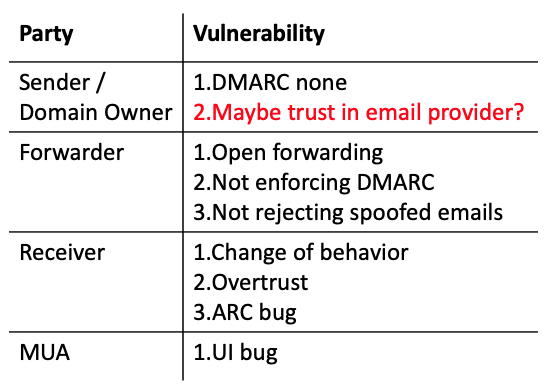
\includegraphics[width=\columnwidth]{graphs/summary_indi_vulnerabilities.png}}
% \centering
% \caption{Summary of Vulnerabilities Identified}
% \label{fig:summary_indi_vulnerabilities}
% \end{figure}

% Please add the following required packages to your document preamble:
% \usepackage{multirow}



% \subsection{Implementation Errors}
% \label{subsec:implementation_errors}
% Finally, in addition to vulnerabilities
% resulting from the design of forwarding and anti-spoofing mechanisms,
% during our experiments we also observed three implementation
% errors. We focus on Zoho's ARC implementation error, which directly
% introduces serious security concerns. The other two errors can be
% abused to help send spoofed email, which we detail in
% Appendix~\ref{sec:implementation_errors_additional}.


% in a subset of our attacks.
% Namely, Gmail's UI indicator bug and Zoho's ARC implementation bug.

% \subsubsection{Every email is legitimate}
% \grant{Hmmm... this subsection really strikes me as a broken implementation, and we might consider moving to Section 4.2}


% \subsubsection*{Zoho's ARC Implementation Error}
% \label{sec:arc}
% % \label{subsubsec:arc_bug}
% As discussed earlier in Section~\ref{sec:measure_forwarding_mechs_and_arc},
% many forwarding approaches break SPF, DKIM, and DMARC authentication.
% To remedy this compatibility issue, a new experimental protocol called Authenticated Received Chain (ARC)~\cite{rfc8617} was recently introduced to preserve email authentication results across multiple forwarders and allow the final recipient to authenticate legitimate email even if they fail DMARC authentication.
% Intermediary forwarders implementing ARC sign their authentication results
% (using new ARC headers) so that the receiver can verify each forwarder's authentication checks.
% If DMARC authentication fails, a receiver can examine the ARC validation chain to determine whether the forwarded email is legitimate~\cite{ARCSpeci1:online}.
% Although ARC can help resolve the compatibility issues with some forwarding implementations and anti-spoofing protocols, it does not remedy the security vulnerabilities presented earlier in this section.
% Additionally, ARC is currently an experimental standard and only
% implemented by a few providers~\cite{rfc8617, ARCSpeci1:online};
% Appendix~\ref{sec:appendix_arc_measurement}
% % and Table~\ref{tab:forwarding_mechs_in_the_wild}
% reports our measurement results about the adoption of ARC among
% the providers we evaluated.
% %\geoff{(will need to be updated if ARC is removed from the table)}
% Nonetheless, during our experiments, we identified attacks that can exploit incorrect ARC implementations to reliably spoof email.

% Among these platforms, many providers only accept ARC signatures from custom lists of ``trusted'' forwarders (Table~\ref{tab:trust_of_arc_between_providers}).
% During our analysis, we discovered that some email providers' implementation of ARC also leads to vulnerabilities, which an attacker can combine with forwarding to spoof malicious emails (\S~\ref{subsec:attack_zoho_arc}).
% Prior work has found that some mail providers, such as Zoho, incorrectly implement ARC~\cite{shen2020weak}.
% For example, when a spoofed email message is forwarded from Gmail to Zoho, Zoho incorrectly reads the ARC headers attached by Gmail. As a result, it incorrectly displays the email as passing DMARC and delivers the email without warnings.
% Echoing this prior work, we found that this vulnerability still existed at Zoho.
% We also found through our experiments that, in addition to Gmail, Zoho also evaluates and trusts ARC headers added by Fastmail (Section~\ref{sec:measure_forwarding_mechs_and_arc}).
% Moreover, by leveraging Fastmail's open forwarding, this flawed ARC implementation could be exploited to spoof email messages to any Zoho user from \emph{any} domain.\footnote{Our work not only led to a patch of this issue after disclosure to Zoho, but also resulted in Zoho adding additional security enhancements to their ARC implementation (Appendix~\ref{sec:disclosure}).  This patch is confirmed by the parallel work of Wang et al.~\cite{wang2022revisiting} that focused on email forwarding under ARC.}


%% \begin{figure}[t]
%%   \centering
%%   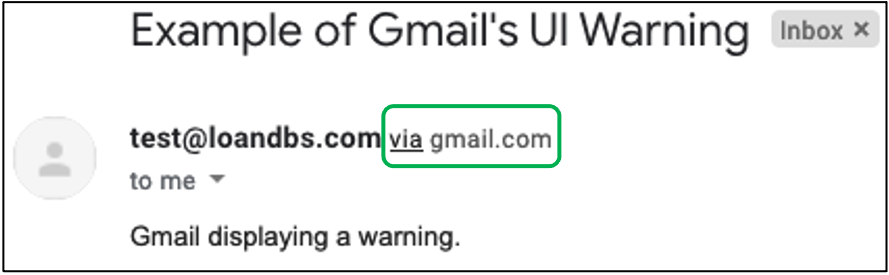
\includegraphics[width=\columnwidth]{graphs/ss_ui_warning_normal.png}
%%   \caption{Gmail's usual UI warning for forwarded mail.}
%%   \vspace*{-0.1in}
%%   \label{fig:gmail_ui_normal}
%% \end{figure}

% However, any such trust implicitly
% assumes that those trusted forwarders have good security practices.
% Unfortunately, as we detail later, this is not always the case, which
% creates additional opportunities for adversaries
% (Section~\ref{subsec:attack_zoho_arc}).


%\input{3.all_forwarding_mechs.tex}

%\input{4.threat_model.tex}


%
% attack summary table in previous section for positioning
%

\section{Attacks}
\label{sec:attacks}
In this section, we demonstrate how an adversary can combine and
exploit the issues
% we have
described in Section~\ref{sec:assumptions} to create attacks that reliably
bypass existing anti-spoofing protections.  In particular, we consider an
attack successful if a spoofed email message is delivered to a
victim's inbox (\ie,  not the spam folder), and yet does not produce a
warning to the user.
Figure~\ref{fig:open_forwarding_attack_screenshot} shows
an example of a successful attack, where a spoofed
email purporting to be from \dns{bush@state.gov} is delivered to a
Gmail user's inbox with no warning indication.

We describe four distinct classes of attacks, summarized in
Table~\ref{tab:summary_attacks}, each of which we have validated
empirically using accounts created at the affected providers.  Some of
these attacks are quite broad --- allowing an attacker to spoof email
to any email recipient purporting to be from tens of thousands of
popular and sensitive domains --- while others are more circumscribed
in their impact.
%
For each of the attacks described below, we refer to the domain an
attacker specifies in their \textsc{FROM} header as the
\textit{spoofed domain}.  We use the terms \textit{spoofed address} to
refer to the full email address appearing in the \textsc{FROM} header
and \textit{forwarding domain} to refer to the domain of the
forwarder.

\begin{figure}[t]
  \centering
%% \centerline{
\includegraphics[width=\columnwidth]{graphs/ss_outlook_open_forwarding.png}}
{
    \setlength{\fboxsep}{0pt}
    \setlength{\fboxrule}{0.5pt}
    \fbox{
\includegraphics[trim=2 2 2 47,clip,width=\columnwidth]{fig/ss_outlook_open_forwarding.png}}
}
%  \vspace*{-0.2in}
  \caption{Example of a successful attack. A spoofed email purporting to be \dns{bush@state.gov} is delivered to a Gmail user's inbox with no warning indicators.
}
%\vspace*{-0.1in}
\label{fig:open_forwarding_attack_screenshot}
\end{figure}


\begin{figure*}[t]
  \centerline{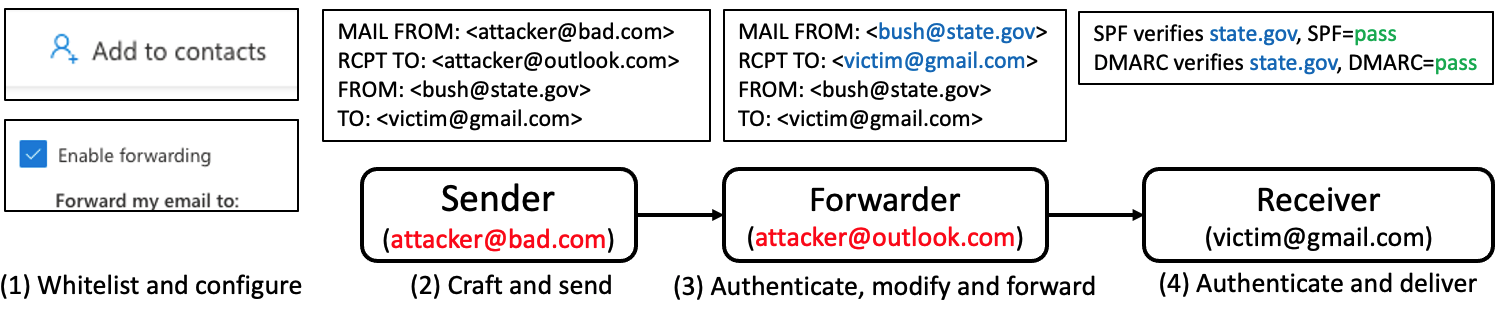
\includegraphics[width=\textwidth]{fig/mech_outlook_open_forwarding.pdf}}
  \centering
  \caption{Example of an SPF Incorporation Attack (\S~\ref{subsec:attack_open_forwarding}) exploiting Outlook's open forwarding to spoof email from domains incorporating Outlook's SPF records (e.g., \dns{state.gov}) to arbitrary recipients.}
  \label{fig:open_forwarding_attack_mechanism}
  %    \vspace*{-0.1in}
\end{figure*}


\paragraph{Threat Models}
For the first three attacks, we assume an adversary controls the
sender and forwarding accounts: they possess a server capable of
sending spoofed email messages (sender) and a personal account with a
specific third-party provider that allows \emph{open forwarding}
(forwarder). For the attack described in
Section~\ref{subsec:attack_none_mailing_list}, we make three
assumptions: (a) that adversaries control a malicious server that can
send spoofed email messages and try to spoof email from a domain that
hosts a mailing list with REM forwarding (e.g., Google Groups,
Listserv and Mailman as described in
Section~\ref{sec:measure_forwarding_mechs_and_arc}), (b) that the spoofed domain
has a DMARC policy of \textsc{None} (all too common); and (c) the
sending email address the attacker wishes to impersonate has
permission to send to the mailing list.

%We validated each of these attacks empirically using
%accounts we created with each of the affected providers.
%Additionally, we have disclosed all of these vulnerabilities to the
%affected providers (Section~\ref{sec:disclosure}).

%We also demonstrate how an adversary can ``launder'' spoofed email
%through mailing lists, such that the resulting spoofed email also
%passes SPF and DMARC validation checks.


%% include email addressed from: (1) any
%% domain that incorporates Outlook's SPF information in their SPF
%% records (\ie, including thousands of high-profile domains such as
%% \dns{state.gov}, \dns{disneyplus.com}, and \dns{qantas.com}),\alex{do we still want to say any domain} (2) any
%% domain, if the recipient is a Zoho user, and (3) any domain with a
%% DMARC policy of none or quarantine (\eg, \dns{alipay.com}), if the
%% recipient is a Gmail user.

%\grant{I'm not sure how I feel about the caveats about specific email provider. They seem to detract / complicate the impact examples and I wonder if others feel the same or see a way to word them more broadly (e.g., in terms of forwarding approaches, rather than specific providers).}
%\geoff{since we have even more qualifiers on the attacks than before (e.g., Alex's note about any domain no longer being accurate), how about if we reduce this part to something on the order of ``in some cases impacting ....''}

% For the remainder of this section, we
% describe each of these attacks in detail and explain what enables each
% to bypass existing anti-spoofing measures.

%Each attack combines vulnerable forwarding features (\S~\ref{subsec:fwding_vuln}) and/or the header rewriting performed by common forwarding approaches (\S~\ref{sec:background:fwdingflow}) to violate security assumptions made by anti-spoofing defenses (\S~\ref{subsec:assumptions}).
%While these defenses would have mitigated spoofing in a direct email transmission settings, the use of forwarding enables successful spoofing attacks.
% For each attack, we describe the steps an attacker performs to successfully spoof an email and explain how forwarding,
% combined with the vulnerabilities from Section~\ref{sec:assumptions} enable the attack to bypass anti-spoofing measures.
 % and will report on their feedback in a final version of this paper.

% In all four attacks, we assume that the adversary controls their own SMTP server for sending spoofed email messages (i.e., the sender is malicious). Additionally, for the first three attacks, we assume that the adversary also controls personal email accounts registered with the forwarder, which is easily done with services like Outlook and Fastmail. For the last attack involving mailing lists, we assume that the adversary knows a target email address within the organization that is allowed to send to the mailing list.


\begin{figure*}[t]
  \centerline{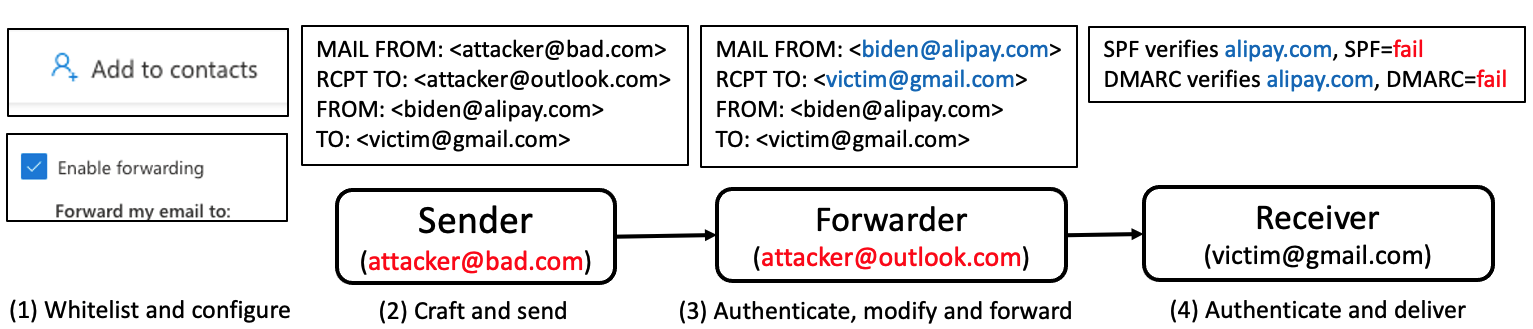
\includegraphics[width=\textwidth]{fig/mech_gmail_via_outlook.pdf}}
  \centering
  \caption{Example of a spoofed email attack exploiting open forwarding and relaxed validation for forwarded email from well-known providers (\S~\ref{subsec:attack_relaxed_forwarding_validation}).
    Note that the spoofed domain, \dns{alipay.com}, has a DMARC policy of Quarantine and thus
    % its traffic
    should not be delivered.}
  \label{fig:mech_gmail_via_outlook}
\end{figure*}


\subsection{Exploiting SPF Incorporation}
\label{subsec:attack_open_forwarding}

% \subsubsection*{Attack Overview}
The first attack we describe exploits five discrete issues:
three security assumptions (\S~\ref{subsubsec:spf_incorporation},~\ref{subsubsec:quarantine_instead_of_reject},~\ref{subsubsec:whitelist}),
the vulnerable \emph{open forwarding} feature that many providers offer (\S~\ref{subsubsec:open_forwarding}),
and the header rewriting performed as part of the PMF and MFEF forwarding approaches (\S~\ref{sec:measure_forwarding_mechs_and_arc}).
Crucially,
%as described in Section~\ref{subsubsec:spf_incorporation},
the rise of large third-party email providers violates SPF's assumption that the set of authorized server IP addresses specified by each domain cannot be used by other domains or external users to send email.
% SPF assumes that set of authentic server IP addresses that each domain specifies cannot be used by other domains or external users to send emails. The rise of third-party providers has challenged this assumption --- many domains now outsource their email services to these third-party email providers.
For example, the owners of domain \dns{state.gov} use Outlook as their email provider.  Thus, email messages sent by \dns{state.gov}'s employees will originate from Outlook's mail servers.
To ensure reliable delivery, such domains routinely add the server IP addresses of their email provider to their own SPF records.
Although intuitive, this configuration creates an overly broad trust assumption: by adding the provider IP addresses to their SPF record, such domains (e.g., \dns{state.gov}) implicitly grant permission for any account hosted by their provider, whether individual or corporate, to send email messages that purportedly come from their domain.
This threat is only prevented because large providers like Outlook do not allow users to arbitrarily set or forge their email's FROM header.

However, we observe that by combining header rewriting from PMF and MFEF and the use of \emph{open forwarding}, attackers can overcome this defense and exploit SPF's violated assumption.
Specifically, this attack allows an adversary to spoof email from domains that incorporate a third-party provider's SPF information in their own SPF record to any recipient, regardless of the domain's DMARC policy.
%absent additional protections.

% Outlook also enables \emph{open forwarding} and uses the MFEF forwarding approach, which provides attackers with a mechanism for sending email messages with forged FROM headers.
% While Microsoft does not provide a mechanism for forging the FROM header, a malicious sender can spoof as arbitrary domain in the FROM header. With open forwarding, an adversary can create an individual Outlook account and use it to redirect an email with a forged FROM header to an arbitrary destination without verification.
% Together, these issues allow an adversary to reliably spoof as any domain that incorporates a third-party provider's SPF information in their own SPF absent some other protection.
% \subsubsection*{Impact}
%\paragraph{Impact}
\paragraph{Scope}
This attack works for domains that include the SPF record of any of six
large email providers (Outlook, iCloud, Freemail, Hushmail, Mail2World and Runbox) in their own SPF records.  Notably, given
Outlook's importance as a third-party provider~\cite{liu2021s}, this
attack allows an attacker to spoof email on behalf of tens of
thousands of popular domains.

Indeed, over 12\% of the Alexa 100K
most popular domains are vulnerable as a result (and almost 8\% of the
top 1M domains).  A cursory examination of this list identified a
range of potentially sensitive domains such as those hosting large
news reporting organizations (\eg, \dns{washingtonpost.com},
%\dns{cbsnews.com},
\dns{latimes.com},
%\dns{slate.com}, \dns{npr.org},
and \dns{apnews.com}),
%\dns{nydailynews.com} and \dns{afp.com}),
financial services (\eg,
%\dns{usbank.com}, \dns{discover.com},
\dns{mastercard.com}, \dns{transunion.com},
%\dns{fidelity.com},
and \dns{docusign.com}),
domain registrars (\eg, \dns{godaddy.com}),
certificate authorities (\eg,
\dns{sectigo.com} and \dns{digicert.com}) and large law firms (\eg,
\dns{perkinscoie.com}).  In addition, 32\% of US \dns{.gov} domains are
vulnerable (including 22\% of the domains used by Federal
agencies).  At the Federal level this includes the majority of US
cabinet organizations (\eg, \dns{state.gov}, \dns{dhs.gov} and
\dns{doe.gov}), a range of security sensitive agencies (\eg,
\dns{odni.gov}, \dns{cisa.gov} and \dns{secretservice.gov}) as well
as those charged with public health and safety (such as
\dns{fema.gov}, \dns{nih.gov}, and \dns{cdc.gov}).
%% \footnote{To say
%%   nothing of other critical government functions such as the funding
%%   of scientific research (\eg  nsf.gov).}
At the state and local
level, virtually all primary state government domains (\eg, \dns{mass.gov})
  are vulnerable (including a broad range of congress, judiciary,
  and law enforcement domains in each state) and over 40\% of all \dns{.gov}
  domains used by cities.\footnote{We have not broadly examined domains representing government offices outside the US, but we note that both \dnsfn{gchq.gov.uk} and \dnsfn{ncsc.gov.uk} are also vulnerable.}


% \footnote{Our estimation suggests that roughly
% 12.4\% of Alexa top $100K$ domains and 38.1\% of \dns{.gov} domains are
% vulnerable to this attack absent some other protection
% mechanism.
% This list includes both popular commercial domains such as \dns{disneyplus.com},  \dns{hulu.com} and \dns{qantas.com} and sensitive domains used by the U.S. government in its official capacity such as \dns{state.gov}, \dns{nsf.gov}, \dns{cdc.gov} and \dns{cisa.gov} among many others.}.


%% %Absent additional per-domain protections by
%% %Outlook(\S~\ref{subsubsec:whitelist}), this attack can be used to spoof any domain that incorporates Outlook's SPF information in their SPF
%% %record, regardless of the domain's DMARC settings (e.g., even with a
%% %policy of Reject).  Additionally, they can successfully deliver this
%% %spoofed email to any recipient at any email provider.
%% %\geoff{revisit: qualify this slightly in light of aa.com}
%% %
%% Figure~\ref{fig:open_forwarding_attack_mechanism} shows an example of
%% this attack using Outlook as the forwarding service. It consists of four stages.
%% %\label{subsubsec:open_forwarding_attack_mechanism}
%% %\alex{Updated the text}\grant{Would it work to incorporate this email forging as part of Stage 1,
%% %perhaps even just as text (Without changing the diagram).
%% %It's a little weird that we list some actions the attacker needs to do, and then talk about ``Stage 1'' and what the attacker does.}
%% An attacker starts by creating a personal account for
%% forwarding (\dns{attacker@outlook.com}), adding the spoofed address
%% (\dns{bush@state.gov}) to the account's ``allowlist'' (thereby
%% preventing any quarantining by Outlook), and configuring the account to
%% forward all email to the desired target (\dns{victim@gmail.com}). In this case, the spoofed domain \dns{state.gov} includes
%% Outlook's SPF record (\dns{spf.protection.outlook.com}) into its own SPF record and has a DMARC policy of \textsc{Reject}. Next, the attacker forges an email that purportedly originates from \dns{state.gov} and sends it to their personal Outlook account. Then, even though the message fails DMARC validation, Outlook will still forward it because the spoofed address is present in the account's allowlist.

  
  
% \subsubsection*{Threat Model and Attack Procedure}
%\paragraph{Attack Procedure}
\paragraph{Example}
%% \alex{another version of the above paragraph that works in the assumptions.}
% (need to reference the figure somewhere)
Figure~\ref{fig:open_forwarding_attack_mechanism} shows an example of
this attack using Outlook as the forwarding service.
An attacker starts by creating a personal account for
forwarding (\dns{attacker@outlook.com}), adding the spoofed address
(\dns{bush@state.gov}) to the account's ``allowlist'' (thereby
preventing any quarantining by Outlook), and configuring the account to
forward all email to the desired target (\dns{victim@gmail.com}). In this case, the spoofed domain \dns{state.gov} includes
Outlook's SPF record (\dns{spf.protection.outlook.com}) into its own SPF record and has a DMARC policy of \textsc{Reject}. Next, the attacker forges an email that purportedly originates from \dns{state.gov} and sends it to their personal Outlook account. Normally, Outlook would quarantine this email because it fails DMARC validation (\S~\ref{subsubsec:quarantine_instead_of_reject}). However, since the spoofed address is present in the account's allowlist, this configuration overwrites the quarantine decision (\S~\ref{subsubsec:whitelist}), and as a result, Outlook would forward the spoofed email to the target.


As per Outlook's MFEF forwarding implementation,
%the
\textsc{MAIL FROM}
%header
is rewritten to match the
\textsc{FROM} header, \dns{bush@state.gov} in our example. Finally, the recipient's mail server receives the forwarded email
and performs authentication checks.
From the recipient's perspective,
the spoofed email passes SPF validation because the
\textsc{MAIL FROM} domain (\dns{state.gov}) lists Outlook's SPF
information in its SPF record, and the forwarding configuration
arranged by the attacker ensures that the recipient receives this
spoofed email from Outlook's servers.
Moreover, this attack also
ensures that DMARC's alignment check succeeds because the
\textsc{MAIL FROM} and \textsc{FROM} domain are both \dns{state.gov}.
%\stefan{I don't think we need the screenshot.  I think they will believe us}
%\alex{nope we need this one}
We validated this attack in practice, consistently sending
spoofed email messages such as the example
shown in Figure~\ref{fig:open_forwarding_attack_screenshot}
to our own Gmail account, where it was delivered to the inbox without warning.\footnote{
Note that we did discover some exceptions in our experiments.
For a small set of high-profile domains that have a DMARC policy of Reject
(\eg, \dnsfn{aa.com}, \dnsfn{foxnews.com} and \dnsfn{ikea.com}), Outlook would
quarantine spoofed email regardless of whether users have added the
spoofed address to their account's allowlist (Section~\ref{subsubsec:quarantine_instead_of_reject}).
We surmise that Outlook applies special protections for a set of high-profile or frequently spoofed domains.
} 
In addition to Outlook, this attack also succeeds with
% five other large email providers:
iCloud, Freemail, Hushmail, Mail2World and Runbox.


\subsection{Abusing Relaxed Forwarding Validation}
\label{subsec:attack_relaxed_forwarding_validation}

% \subsubsection*{Attack Overview}
The second attack exploits the fact that many email providers apply relaxed validation policies to forwarded mail (\S~\ref{subsubsec:relaxed_validation}), particularly when messages arrive from well-known mail providers.
When combined with open forwarding, an attacker can abuse this behavior
to spoof email from any domain that has a DMARC policy of
%\geoff{is an and valid here?}\alex{yes. for gmail it is None and Quarantine}
\textsc{Quarantine} (or \textsc{None}) to any mail server that applies these relaxed measures (\eg, Gmail and Outlook).  Recall that, in the absence of forwarding, attackers cannot spoof email from a domain with a DMARC policy of \textsc{Quarantine}.
Provider-specific defenses, such as when Outlook quarantines any email that fails DMARC (\S~\ref{subsubsec:dmarc_none}), will also stop such direct, single-hop attacks.

\begin{figure*}[t]
\centerline{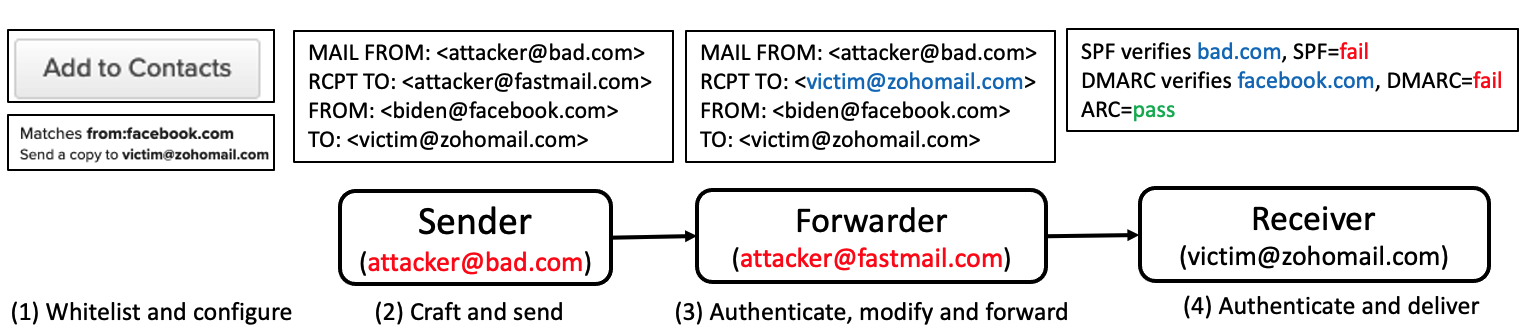
\includegraphics[width=\textwidth]{fig/mech_zoho_arc.pdf}}
\centering
\caption{Example attack that exploits Zoho's
vulnerable ARC implementation and  open forwarding to
  spoof email from arbitrary domains to any Zoho recipient (\S~\ref{subsec:attack_zoho_arc}).}
\label{fig:mech_zoho_arc}
%\vspace*{-0.1in}
\end{figure*}

% \subsubsection*{Impact}
%\paragraph{Impact}
\paragraph{Scope}
As described earlier in Section~\ref{subsubsec:relaxed_validation}, Gmail and Outlook use relaxed validation checks for forwarded email.
We find that an adversary can mount this attack against users with
Gmail/Outlook email accounts as well as users who use GSuite and Outlook 365 for email services.\footnote{Mail.ru also uses relaxed validation, but since it is only applied to email forwarded via Gmail, which does not allow open forwarding, this attack does not work for Mail.ru.}
%As a result, this attack impacts
% who together have
% roughly 1.9 billion users worldwide~\cite{GmailWik42:online, Outlookc33:online}
% when taking into account both users with
% Gmail/Outlook email accounts, as well as all users who use GSuite and
% Outlook 365 for email services (who are also vulnerable)

% \subsubsection*{Threat Model and Attack Procedure}
%\paragraph{Attack Procedure}
\paragraph{Example}
Figure~\ref{fig:mech_gmail_via_outlook} illustrates the steps of this
attack using an example where the adversary creates a personal Outlook
account to forward spoofed email messages to Gmail recipients.  First,
the adversary selects a spoofed email address from a domain with a
DMARC policy of \textsc{Quarantine} or \textsc{None} (we use \dns{alipay.com} in this example, a prominent Chinese payment company), adds the address
to their forwarding account's allowlist, and configures their
forwarding account to send email to the victim (recipient).  Like the
first attack, the attacker then sends a message from this spoofed address
to their forwarding account, which is then forwarded to the recipient.

When the final recipient's mail server receives
the email, the server will observe that the email comes from a
``well-known'' provider, apply its relaxed validation checks, and
successfully deliver the email to the recipient's inbox (even though
the spoofed email fails normal SPF and DMARC checks).\footnote{Additionally, we note that Gmail would usually display a UI warning for forwarded email messages. However, no UI warning is displayed for this email due to a bug detailed in Appendix~\ref{subsec:ui_bug}.}
%\alex{The part that talks about the UI bug}
%We verified this attack, and Figure~\ref{fig:ss_gmail_via_outlook} in the Appendix shows one such spoofed message delivered to GMail without security warnings.


\subsection{Targeting ARC Vulnerabilities}
\label{subsec:attack_zoho_arc}
% \subsubsection*{Attack Overview}
The third attack allows an adversary to deliver spoofed email messages
from arbitrary domains to Zoho users.  This attack exploits Zoho's
vulnerable implementation of the experimental Authenticated Received
Chain (ARC) protocol~\cite{ARCSpeci1:online}, which was first
documented by Shen et al.~\cite{shen2020weak}. Due to this bug, Zoho
incorrectly reads ARC headers and will deliver arbitrary email
messages with ARC headers added by providers such as Gmail and
Fastmail to the recipient's inbox without any warning.  However, we
show that this issue is not limited to interactions between Gmail and
Zoho customers.  We demonstrate how further issues, including the fact that
Zoho trusts and (incorrectly) reads ARC headers added by Fastmail
(Appendix~\ref{sec:arc_adoption_and_trust}), open forwarding
(\S~\ref{subsubsec:open_forwarding}), and several forwarding
assumptions (\S~\ref{subsubsec:quarantine_instead_of_reject},
\S~\ref{subsubsec:whitelist}), can be combined with the underlying ARC
vulnerability to allow an adversary to deliver spoofed email messages
from arbitrary domains to arbitrary Zoho users.

This attack again highlights the fact that email security protocols
are distributed and independently-configured components, where
vulnerable decisions by one party incur harm to downstream recipients
but not necessarily to their own users.  Notably, the actions taken
by one provider (e.g., Fastmail) can unexpectedly undermine the
security of users on another platform (e.g., Zoho).

%This attack works by combining several vulnerabilities: Zoho's vulnerable ARC implementation (more details below), 

%One main vulnerability exploited in this attack is Zoho's vulnerable
%implementation of the experimental Authenticated Received Chain (ARC)
%protocol~\cite{ARCSpeci1:online}, which was first documented by Shen
%et al.~\cite{shen2020weak}. Due to this bug, Zoho incorrectly reads
%ARC headers and will deliver arbitrary email messages with ARC headers
%added by providers such as Gmail and Fastmail to the recipient's inbox
%without any warning.

%To make this attack work, an adversary needs to
%exploit multiple different vulnerable forwarding assumptions and
%features, in addition to the flaw in Zoho's ARC implementation.
%We note that our work has not only led
%to a patch resolving this issue after disclosure to Zoho, but also
%resulted in Zoho adding additional security enhancements to their ARC
%implementation (Section~\ref{sec:disclosure}).
%\stefan{
%\grant{I'm commenting out the list of vulnerable things below because it seems redundant with both the intro paragraph and the attack description.}

% Importantly, several forwarding assumptions and open forwarding are required for this attack to work, in addition to Zoho's buggy ARC implementation. Namely, the attack we demonstrate in this section exploits that Fastmail allows open forwarding (Section~\ref{subsubsec:open_forwarding}), that Fastmail allow users to overwrite DMARC decisions through whitelisting (Section ~\ref{subsubsec:whitelist}), that Fastmail does not reject spoofed email messages addressed from domains with DMARC policy \textsc{REJECT} (Section~\ref{subsubsec:quarantine_instead_of_reject}), and that Zoho (incorrectly) reads ARC headers added by Fastmail (Appendix~\ref{sec:appendix_arc_measurement}). We provide more details in the example below.

%\paragraph{Impact}
\paragraph{Scope}
Our experiments show that this attack can target arbitrary users of Zoho, which is estimated to have more than 10 million users~\cite{Celebrat69:online}.

 % To some estimate~\cite{Celebrat69:online}, this attack impacts more than 10 million users.

%% \begin{figure}[t]
%% \centering
%% \includegraphics[width=\columnwidth]{graphs/mech_google_groups.pdf}
%% \centering
%% \caption{Spoofed email attack that abuses mailing lists like Google Groups (\S~\ref{subsec:attack_none_mailing_list}).}
%% \label{fig:google_groups_mech}
%% \vspace*{-0.1in}
%% \end{figure}

%% (geoff: since we have extra space in the camera ready version, I
%% resized this figure so that its elements are roughly the same size
%% as the first three attack figures.  feel free to undo if you don't
%% like it)
\begin{figure*}[t]
\centering
\includegraphics[width=\textwidth]{fig/mech_google_groups.pdf}
\centering
\caption{Spoofed email attack that abuses mailing lists like Google Groups (\S~\ref{subsec:attack_none_mailing_list}).}
\label{fig:google_groups_mech}
%\vspace*{-0.1in}
\end{figure*}




% \subsubsection*{Threat Model and Attack Procedure}
%\paragraph{Attack Procedure}
\paragraph{Example}
Figure~\ref{fig:mech_zoho_arc} shows the mechanics of this attack
%,
%which also consists of four phases,
in the context of an attacker with a forwarding account on Fastmail who targets a recipient on Zoho.

First,
%, as in the first attack,
the adversary creates a Fastmail account for forwarding, adds their spoofed address
(\dns{biden@facebook.com}) to their allowlist, and configures their
account to forward all mail to the target user at Zoho
(\dns{victim@zohomail.com}).
Second, the adversary crafts and sends
spoofed email from their own servers (\eg, \dns{attacker@bad.com})
to their forwarding account at Fastmail.
Third, although this email will fail anti-spoofing validation, Fastmail will still faithfully forward it to the target user at Zoho due to the sender's presence on the user's allowlist (exploiting the security assumption discussed in \S~\ref{subsubsec:whitelist}). 
As part of the forwarding process,
Fastmail will modify the RCPT TO header and add corresponding ARC headers to the
spoofed email.
Finally, upon receiving the forwarded email, Zoho's mail server will perform DMARC validation.
Although the spoofed email will fail SPF and DMARC checks,
Zoho's vulnerable ARC implementation
will misinterpret the ARC headers that Fastmail attached (Appendix~\ref{sec:arc_adoption_and_trust}).
As a result, Zoho will treat the email as passing
DMARC and deliver the spoofed message to the victim's inbox. We end by noting that this attack would not have worked for domains with DMARC policy \textsc{Reject} had Fastmail rejected spoofed email messages addressed from such domains (\S~\ref{subsubsec:quarantine_instead_of_reject}).
%Figure~\ref{fig:ss_zoho_arc} in the Appendix illustrates that this attack succeeds without any security warnings, even though the spoofed domain in our experiment, facebook.com, has a DMARC policy of \textsc{reject}. 

% \begin{figure}[t]
%   \centerline{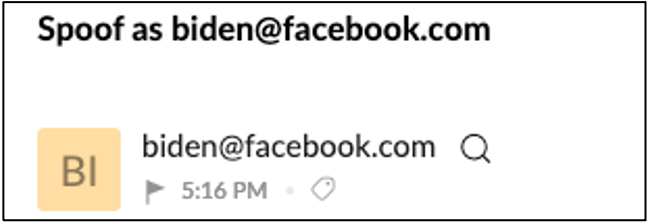
\includegraphics[width=\columnwidth]{graphs/ss_zoho_arc.png}}
%   \centering
%   \caption{An email spoofing \dns{biden@facebook.com} via Fastmail.}
%   \label{fig:ss_zoho_arc}
%   \end{figure}

%Figure~\ref{fig:ss_zoho_arc} in the Appendix illustrates that this attack succeeds without any security warnings, even though the spoofed domain in our
%experiment, \dns{facebook.com}, has a DMARC policy of \textsc{Reject}.



% \subsubsection*{Impact and Mitigation}
% Among providers that we studied, this attack affects customers with
% Zoho email addresses or using Zoho email services,\footnote{We
%   speculate that the above attack also works for customers using Zoho
%   email services, but we are not able to verify this because we are
%   not a Zoho customer.} which together compromise more than 10 million
% potential victims~\cite{Celebrat69:online}.

% However, the attack depends on the existence of providers that allow
% open forwarding and that the receiving provider misinterprets ARC
% headers.  Eliminating either of these factors would foreclose the attack.


\subsection{Abusing Mailing Lists}
\label{subsec:attack_none_mailing_list}

% \subsubsection*{Attack Overview}
The final attack allows an adversary to abuse the forwarding process
used by mailing lists so that spoofed email, which would otherwise
fail DMARC authentication checks, successfully passes both SPF and
DMARC validation.
This attack targets domains with a weak DMARC policy of \textsc{None},
and exploits the way in which many mailing lists rewrite email headers during their forwarding process.
Concretely, this attack allows an adversary to abuse REM header rewriting (\S~\ref{sec:measure_forwarding_mechs_and_arc}) to launder spoofed email through mailing lists such that the forwarded email appears as if it originated from the legitimate sender, even though the original email fails DMARC authentication.\footnote{One such attack used to distribute phishing messages at our institution was part of the impetus for this study.}

% successfully spoof email from any address within an
% organization that uses a vulnerable mailing list service;
% the header rewriting performed by mailing lists makes the spoofed email appear as if originated from the legitimate sender.
% As a result, the attack takes advantage of the header rewriting
% performed by mailing lists to have the spoofed email's headers appear
% as if it originated from the legitimate sender.
%% \geoff{does Sec 4
%%   discuss why mailing lists are designed to work this way, e.g., why
%%   it might have been reasonable for them to work this way?}\alex{Will
%%   add the movitation behind how mailing list operates in sec 2/3,
%%   revisit this later.}

% \subsubsection*{Impact}
%\paragraph{Impact}
\paragraph{Scope}
Our experiments show that attackers can
conduct this attack across all four popular mailing list services: Google
Groups, Mailman, Listserv, and Gaggle.

This attack only affects organizations that use a mailing list configured under their own domain name, and with a DMARC policy of \textsc{None} for their (sub)domain.
While these requirements appear restrictive, prior
work has found that many organizations
(such as major U.S.\ universities) have exactly this configuration~\cite{hutowardsunderstanding}.
Indeed, in querying \dns{.edu} and
\dns{.gov} domains, roughly 10\% of all \dns{.edu}
domains and 5\% of all \dns{.gov} domains are potentially susceptible to this attack.\footnote{As examples, Yale University operates \dnsfn{yale.edu} with a DMARC policy of \textsc{None} and hosts multiple mailing lists using Mailman, and the State of Washington operates a range of mailing lists using Listserv and whose \dnsfn{wa.gov} domain also has a DMARC policy of \textsc{None}.}

Additionally, for mailing lists like Gaggle that do not enforce DMARC
checks before forwarding (Appendix~\ref{subsec:no_dmarc}), this attack affects every organization using their services,
even when the domain has adopted stronger DMARC policies.

% We contribute to the security analysis of mailing lists by
% identifying three possible attacks against all four mailing lists.
% In all three attacks, a spoofed email would be properly forwarded by a mailing list and pass DMARC checks after being forwarded, which makes it very trustworthy. The attacks in this section exploit forwarding mechanisms used by mailing lists and the known weak DMARC policy none.
%
% \alex{HELP NEEDED: I don't how to summarize the three attacks in
% one sentence. See the details below}



% \subsubsection*{Threat Model and Attack Procedure}
%\paragraph{Attack Procedure}
\paragraph{Example}
%In this attack, adversaries control a malicious server that can send spoofed email messages and aim to spoof email from a domain that hosts a mailing list with REM forwarding (Section~\ref{sec:background:fwdingflow}),
%such as Google Groups, Mailman, and Listserv.
%For this attack to work, the spoofed domain must have a DMARC policy of None,
%and the sending email address the attacker wishes to impersonate must have permission to send to the mailing list.
% This attack assumes that only the sender is malicious --- that the adversary controls a server capable of sending spoofed email messages. Additionally, we assume that the domain the adversary wishes to spoof (\dns{univ.edu}) hosts a mailing list with one of these providers,
% such as \dns{list@univ.edu} if they use Google Groups, or \dns{list@listserv.univ.edu} if they use Listserv.
% For this attack to work, \dns{univ.edu} must have a DMARC policy of none,
% and the \dns{univ.edu} email address the attacker wishes to impersonate must have permission to send to the mailing list.
Figure~\ref{fig:google_groups_mech} describes an example of this attack
using Google Groups.
First, an attacker selects a target email address (\dns{someone@univ.edu}) to impersonate in their spoofed email,
and sends the spoofed message from their malicious server to the organization's mailing list (\dns{list@univ.edu}).
Although the email fails DMARC validation,
the mailing list will still accept the message (because \dns{univ.edu}
has a DMARC policy of \textsc{None}).
As part of REM forwarding, the mailing list will rewrite the
\textsc{MAIL FROM} header such that its domain matches the mailing
list's domain, and then forward the email to the list's members.
%(\eg, a new \textsc{MAILFROM} address of
%\dns{xyz@univ.edu}).\footnote{The exact username (the ``xyz'' part) in
%  the \textsc{MAILFROM} address after rewriting depends on the
%  specific implementation.}
As a result, when a recipient's server receives the message it will
successfully pass SPF validation since the domain of the rewritten
\textsc{MAIL FROM} (\dns{univ.edu}) allows the mailing list to send on
its behalf.
Moreover, the spoofed message will also pass DMARC alignment checks,
since the rewriting performed during REM forwarding
ensures that the \textsc{MAIL FROM} and \textsc{FROM} domains are
identical.\footnote{Note that while our examples show this attack
using the organization's top-level domain, it is also effective for
any of the organization's subdomains (if the subdomains also have
DMARC policy \textsc{None}) due to DMARC's inherent relaxed alignment policy.}

During our experiments, we also observed that some mailing list
services, such as Gaggle, do not enforce DMARC policies at all
(Appendix~\ref{subsec:no_dmarc}).
This lack of enforcement allows the attack to succeed regardless of the spoofed domain's DMARC policy.
We provide more details in Appendix~\ref{sec:append_mailing_list_details}.









%\input{5.sender.tex}
%\input{6.forwarder.tex}
%\input{7.receiver.tex}
%\input{deliverability_without_arc.tex}
%\input{security_without_arc.tex}
%\input{deliverability_with_arc.tex}
%\input{security_with_arc.tex}
%\input{8.ui.tex}
%\section{Ethics}
\label{sec:ethics}

We believe our work, which deals with public data, no identified
individuals and a simple means for identifying attacks on crypto token
transfer bridges (and potentially preventing such attacks in the
future), has very low ethical risk and significant upside. Moreover, I have attempted to disclose significant suspicious bridge
transactions to appropriate bridge operators (yet with limited
success as most of the bridges have ceased operations). Lastly, I will make our code and data available upon publication.
% 
% We strictly use public data and to
% the extent that I identify outcomes (e.g., attacks) they are at the
% granularity of bridges and blockchains, not individuals.

% As well,


% Considering the Menlo report principle of ``Respect for Persons'', we
% are not dealing with, nor do I attempt to analyze, data at the
% granularity of individual persons.  We strictly use public data and to
% the extent that I identify outcomes (e.g., attacks) they are at the
% granularity of bridges and blockchains, not individuals.  Similarly,
% with respect to the principle of ``Justice'', I have no reason to
% believe that our analysis discriminates at the level of persons or
% distinct groups of persons --- all users of bridges should benefit
% equally (excepting criminals).  On the topic of ``Respect for Law and
% Public Interest'', I are engaging with existing public data, I have
% documented our methods clearly and I are careful to limit our factual
% statements to those for which I have evidence.  As well, I have made
% a point to disclose significant suspicious bridge transactions to appropriate
% bridge operators.


% We believe our work, which deals with public data, no identified
% individuals and a simple means for identifying attacks on crypto token
% transfer bridges (and potentially preventing such attacks in the
% future), has very low ethical risk and significant upside.  However,
% in the interest of due diligence, I provide a more thorough
% justification of this position following the Menlo Report principles
% as indicated by the USENIX Security call.

% Considering the Menlo report principle of ``Respect for Persons'', we
% are not dealing with, nor do I attempt to analyze, data at the
% granularity of individual persons.  We strictly use public data and to
% the extent that I identify outcomes (e.g., attacks) they are at the
% granularity of bridges and blockchains, not individuals.  Similarly,
% with respect to the principle of ``Justice'', I have no reason to
% believe that our analysis discriminates at the level of persons or
% distinct groups of persons --- all users of bridges should benefit
% equally (excepting criminals).  On the topic of ``Respect for Law and
% Public Interest'', I are engaging with existing public data, I have
% documented our methods clearly and I are careful to limit our factual
% statements to those for which I have evidence.  As well, I have made
% a point to disclose significant suspicious bridge transactions to appropriate
% bridge operators.

% Finally, on the topic of ``Beneficence'', we
% identify the three sets of stakeholders in our work.  These include
% the past and (potential) future victims whose investments, both direct
% and indirect, via token transfer bridges have been undermined by
% large-scale thefts from these services.  In addition, other
% stakeholders include bridge operators and, finally, the criminal actors who
% derive income from vulnerabilities in bridges.  We argue that our
% retrospective analysis creates no direct new harm for any parties ---
% these attacks have already happened.  For bridge operators, our
% analysis may create some potential liability in supporting a civil
% claim of poor stewardship, but at the same time our documentation of
% the widespread nature of this problem provides a ``common practice''
% defense.  Some of the unilateral transfers I have documented, if they
% were illegitimate (which I do not know), could also create liability
% for bridge operators, but I believe this potential harm is balanced
% against the interest of investors in transparency and fairness in
% operating financial services.  Finally, for our proposed real-time
% analysis approaches, if these were adopted by bridge operators, it
% could foreclose a broad range of attacks.  We admit that this outcome
% could harm our criminal stakeholders as it might deny them of an
% important income stream.  Knock on effects could include a reduction
% in revenues for online crypto money laundering services and Lamborghini
% dealerships, but I believe this is well-justified by the concordant
% reduction in victimization.




\section{Ethics and Disclosure}
\label{sec:disclosure}
When sending spoofed email messages in our experiments,
I took deliberate steps to avoid impacting any real users.
First, I only sent spoofed email messages to accounts that I created ourselves.
Second, I initially tested each attack by spoofing domains that I created and controlled for this research.
Once I established that our attacks could succeed using these test domains,
I ran a small set of experiments that spoofed email from real domains (to validate the absence of any unforeseen protection);
however, these email messages were only sent to our test accounts and did not spoof existing, legitimate email addresses from these domains.
Finally, all of our email messages contained innocuous text (e.g., ``a spoofed email'') that would not themselves cause harm.
% even if a message had somehow been misdelivered,
% all of our messages contained innocuous content and thus was unlikely
% to cause harm.

I have disclosed all of the vulnerabilities and attacks to the
affected providers. As of the time of publication, I have received
affirmative feedback from all affected providers and I summarize our
current understanding of their present state here. Zoho has not only
patched the issue with their ARC implementation (also confirmed by
Wang et al.~\cite{wang2022revisiting}, who conducted their
measurements after the patch) and awarded us a bug bounty, but is also
further augmenting the security of its ARC implementation. Microsoft
confirmed the vulnerabilities (with severity ``Important'', the
highest severity assigned to email spoofing bugs) and awarded us a bug
bounty. They have partially fixed the issues by rejecting spoofed email
messages purporting to be from domains that have a DMARC policy of
\textsc{Reject}~\cite{hotmailreject}.
Gaggle confirmed the issues I flagged and stated that they would
start enforcing DMARC. Gmail fixed the issues I reported.  iCloud
partially fixed the issues I reported by not forwarding email
messages that fail DMARC authentication (except for domains with DMARC
policy \textsc{None}). Hushmail fixed the issues I reported by not
forwarding email messages that fail DMARC authentication. Freemail
fixed the issues I reported by not forwarding spoofed email messages
from domains that are their customers. Mail2World attempted to fix the
issues by using spam filters and remains vulnerable. Runbox did not
view the issues I reported as vulnerabilities. Instead, they consider
monitoring account activities post-complaints sufficient.
% I will report on the full set of disclosure feedback and outcomes in the final version of this paper.


%\input{mitigations.tex}

\section{Discussion and Mitigation}
We end by summarizing the root causes of the issues I discovered, and discuss potential mitigation strategies.

\subsection{Discussion}
In this work, I examine the complexities introduced by email forwarding to email security. We identify a diverse set of email forwarding mechanisms, assumptions, and features, and demonstrate how they can be combined together to perform evasion attacks. These attacks highlight four fundamental issues.

First, as already demonstrated in prior work and further highlighted in this chapter, email security involves distributed, optional, and independently-configured components implemented by different parties. In such an architecture, the
``authenticity'' of an email is commonly determined by the party with the weakest security settings. While traditionally email is sent directly from sender to receiver, forwarding involves three parties instead of two and introduces an extra layer of complexity. As I have shown, a vulnerable forwarder can jeopardize the security of downstream recipients that do not have problematic configurations or implementations. This inversion of
incentives and capabilities naturally complicates
mitigating forwarding vulnerabilities.

A second problem is that email forwarding has never been fully standardized, despite the longevity and popularity of its use. A lack of standardization has led to ad-hoc implementation decisions, each making different assumptions.
% Indeed, through our large-scale measurements, I identify a diverse set of email forwarding mechanisms, assumptions and features.
This ad-hoc nature of implementations makes it challenging to perform both manual security analysis (analyzing individual implementation decisions is a non-trivial task even for experts) and automated testing (any such tool needs to account for the specific implementations of each provider).
% reasoning about them challenging
% This is in addition to the challenge that there exists no universal dataset of all implementation choices.
% While our large-scale empirical measurements have
% addressed parts of this issue, 
While our large-scale empirical measurements have been able to reveal
the assumptions made by providers and their implications, it has
required substantial manual work.  This manual process is a reflection
of the fact that there exists no unified framework or standard for
implementing email forwarding.
% Any tool that seeks to automate the process needs to adapt to the specific implementations of each provider. In addition, it needs to handle a variety of other issues that are orthogonal to forwarding, such as automatic account creation, authentication, and bypassing anti-bot defenses. All these issues are research topics by themselves.


A third issue is that email is a large, slowly-evolving ecosystem with a wide range of legacy systems and protocols that need to be accommodated.
One example I highlight is the ``outdated'' assumption made by SPF (\S~\ref{subsubsec:spf_incorporation}). When SPF was first designed in the early 2000s, it was common practice for each domain owner to maintain their own mail infrastructure. However, this assumption is obsolete in the modern era, as many domains outsource their email services to third-party providers such as Outlook and Google~\cite{liu2021s}. These large providers often share the same email infrastructure across all customers (both business and personal accounts), violating the assumptions made by SPF. 
To mitigate the risks this reality poses to SPF, providers 
usually prevent users from setting arbitrary values in their FROM header. However, past literature has shown that this defense is not always implemented correctly~\cite{chen2020composition}. We build on top of this prior work by identifying a new attack that can circumvent existing defenses through forwarding (\S~\ref{subsec:attack_open_forwarding}).

Last but not least, the intrinsic nature of email forwarding is to transparently send an existing message to a new address ``on behalf'' of its original recipient --- a goal very much at odds with the anti-spoofing function of protocols such as SPF and DMARC. As such, a range of ad-hoc decisions have been made to increase the deliverability of forwarded email messages, such as using the REM+MOD forwarding mechanism (\S~\ref{sec:measure_forwarding_mechs_and_arc}), treating forwarded messages specially (\S~\ref{subsubsec:relaxed_validation}), and adding DKIM signatures to forwarded messages (\S~\ref{subsubsec:unsolicited_dkim}). As I have demonstrated, 
these decisions can fail to foresee unexpected interactions that lead to vulnerabilities, even with a lot of deliberation.

\subsection{Mitigation}
The attacks I demonstrate highlight the complicated interactions
between email forwarding and existing anti-spoofing mechanisms. We start by reviewing short-term mitigations that could reduce some of the most significant risks I have uncovered. We then discuss challenges in developing more comprehensive solutions, which would require significant changes in either
protocol or operational practices.

A core issue I highlight in this chapter is the ability to forward spoofed email messages to arbitrary recipients, a critical element in each
of the first three attacks in Section~\ref{sec:attacks}. To mitigate this issue, providers could either block spoofed email messages from being forwarded, or enforce that a forwarder can only forward to accounts under their control by requiring explicit confirmation (similar to
the online domain validation used by modern certificate authorities). However, I note that either approach comes with a usability tradeoff, and different providers make choices based on their considerations. Indeed, providers like Gmail and Mail.ru opted for the former option, while others like iCloud and Hushmail opted for the latter.



% allows users to forward spoofed email messages to arbitrary recipients, while Outlook blocks such forwarding~\cite{hotmailreject}.  We also note that while blocking spoofed email messages from being forwarded would protect downstream recipients, it would also break benign forwarding.  For example, a user forwarding a message from a friend to a colleague would be blocked by such a defense. 


% First, I recommend that all mail service providers disable \emph{open
%   forwarding}, and instead require explicit confirmation that the
% forwarding recipient is under the control of the forwarder (similar to
% the online domain validation used by modern certificate authorities). 
% This requirement would prevent the laundering that is a critical element in each
% of the first three attacks in Section~\ref{sec:attacks}.

% Next, a core assumption made by downstream providers is that upstream providers do not forward spoofed email messages. Blocking spoofed email messages from being forwarded is .

As well, I advocate that providers
should enforce a domain's DMARC \textsc{Reject} policy when specified, rather
than substituting a weaker policy.  If Outlook rejected spoofed
email messages from such domains, the impact of the first attack
exploiting SPF incorporation
would
narrow substantially. We understand that Outlook has plans to take such action in the future~\cite{hotmailreject}.


Unfortunately, all the defenses described above reflect a
case of misaligned
%harms
incentives: the recipients of spoofed email (\eg, spam and phishing)
cannot implement this change, but instead need to rely on the entire
ecosystem of providers and forwarding services to adopt such defenses. 

Email providers can also mitigate the second attack (\S~\ref{subsec:attack_relaxed_forwarding_validation}) by eliminating
relaxed validation policies.  This approach would protect their users
from receiving spoofed email without relying on changes by other
platforms or services.  However, to prevent benign forwarding from
breaking will likely require providers to then implement ARC
validation (which in turn places ARC implementation requirements on
external forwarders).

 % Finally, while relaxed validation certainly helps increase the
%deliverability of forwarded email messages, I recommend implementing
%ARC and stick with DMARC policy when possible.

For the final attack (\S~\ref{subsec:attack_none_mailing_list}) that exploits mailing lists, potential mitigations trade usability for security.
% As for the attack on mailing lists, there exists two types of defense mechanisms that trade usability for security.
First, list owners can turn on message moderation and set their mailing lists to be private.
While these measures increase the difficulty of performing email spoofing attacks, they do not rule out the attack entirely. A dedicated attacker might
nonetheless identify a member of the mailing list and craft an email
that fools a list's moderator.
Second, some mailing list services, such as Listserv, support confirm-before-send~\cite{OnmyLIST7:online}, which requests confirmation from the (true) sender address before delivery.  While this mechanism would impose significant overheads in general, these costs might be acceptable by limiting this confirmation requirement to incoming email that fails DMARC authentication checks.

In addition to the short-term mitigations mentioned above that are
specific to forwarding, others~\cite{chen2020composition,shen2020weak}
have proposed solutions such as improving UI notification, building
better testing tools, and revising RFC standards, which are also
important to consider. Additionally, the newly proposed ARC protocol
may also help mitigate some of the issues I have uncovered. However,
ARC is still in the early stages of development and deployment, 
its details are yet to be fleshed out and its effectiveness in
practice remains to be seen.
% \alex{and it may introduce other unexpected issues.} \grant{I think this last bit is a little speculative and there are enough caveats without it.}

Lastly, I note that comprehensively fixing email forwarding would
require a more fundamental set of changes (e.g., redesigning the
entire suite of email security protocols), which will face significant
deployment challenges given the current state of the email ecosystem.
Chief among these challenges is that any new solution designed to fix
forwarding must address backwards compatibility, a task complicated by
email's forty-year-old ecosystem of varied protocols, implementations
and use cases.  Specifically, one must carefully consider how any new
approach interacts and interoperates with existing systems (e.g., mail
providers and filtering service providers) and protocols (e.g., SPF,
DKIM and DMARC).  While security might be enhanced by embracing a
single standard approach to forwarding (e.g., when a message
should be forwarded, what forwarding mechanisms should be used, what
information should be added to forwarded messages, and how the
receiving account should be verified), any such choice will inevitably
  align well with certain providers and conflict with those whose
  existing services have made different choices or who operate under
  different threat models.  Finally, it is not enough to merely
  standardize new protocols, but one must then also incentivize and
  coordinate their universal deployment and operation.  Thus, while
  such an aspirational goal is worthy of attention, it seems likely
  that email will continue to benefit from incremental and reactive
  improvements, such as those discussed earlier, for some time yet.


\section{Conclusion}
\label{sec:discussion}
Internet-based email has been in use since the early 1970s
and the SMTP protocol has been in use since 1980.  It is arguably the
longest-lived text-based communication system in wide use.
Unsurprisingly, its design did not anticipate the range of challenges
we face today and, because of its central role, we have been forced
to upgrade email protocols slowly and with deference to a wide range
of legacy systems and expectations. Perhaps nowhere is this more clear
than around the issue of authentication.  Email protocols have no
widely-used mechanism for establishing the authenticity of sender
addresses, and thus we have focused on authenticating the domain
portion of the email address (largely motivated by spam and phishing).

In this work, using large-scale empirical measurements of 20 prominent email forwarding services, we identify a diverse set of email forwarding mechanisms, assumptions, and features, and demonstrate how they can be combined together to perform four types of evasion attacks. While we are the first academic work to document these attacks, retrospectively examining Mailop~\cite{Mailop96:online}, a prominent mailing list for mail operators, we have also found traces~\cite{RealTraces} of real-world attacks that are similar to what we reported in this chapter. 

The attacks we document exploit four kinds of problems. One fundamental issue is that email security protocols are
distributed, optional, and independently-configured components. This creates a large and complex attack surface with many
possible interactions that cannot be easily anticipated or
administered by any single party. A second problem is that email forwarding was never standardized, leading to ad-hoc implementation decisions that might be vulnerable. A third problem is that protocol assumptions for SPF are grounded at a
point in time and have not been updated as practices have changed. Domains now out-source their mail service to large providers that share mail infrastructure across customers, undermining assumptions made in the design of SPF. Lastly, the intrinsic nature of email forwarding is to transparently send an existing message to a new address ``on behalf'' of its original recipient. 
This creates complex chain-of-trust issues that are at odds with implicit assumptions that mail is sent directly from sender to receiver. Indeed, it is this complication that has driven the creation of ARC.


While there are certain short-term mitigations (\eg, eliminating the use of
open forwarding) that will significantly reduce the exposure to the
attacks we have described here, ultimately email requires a more
solid security footing if it is to effectively resist spoofing
attacks going forwards.


Chapter~\ref{chap:eurosp23}, in part, is a reprint of the material as it appears in Proceedings of the IEEE European Symposium on Security and Privacy 2023. Enze Liu, Gautam Akiwate, Mattijs Jonker, Ariana Mirian, Grant Ho, Geoffrey M. Voelker, and Stefan Savage. The dissertation author was the primary investigator and author of this paper.


%first shed light on the security issues of component-based defense. We
%further examine this issue in the context of email forwarding. For
%example, as we mentioned in Section~\ref{subsec:sender_vulnerability},
%certain providers accept spoofed email messages from domains with
%DMARC none. They rely upon other components (\eg, UI indicators) to
%warn users. As shown by prior work, such components may not exist,
%especially if users are using third-party providers. In this work, we
%further demonstrate such issues in the co


%\alex{can merge with conclusion}
%The attacks we identified have shared some of the high-level concepts. We outline three sources of issues that manifest in the overall picture.
%\alex{Some of the key issues: protocol design vs protocol use; post-hoc protocols not work well for existing use (forwarding); chain of trust; component-based defense; Lack of Standard for forwarding; }

%\paragraph{Inconsistencies between the design and the use of a protocol}
%Protocols designed in the past might make assumptions that do not hold nowadays. Some of the security protocols (\eg, SPF) were designed in the early 2000. SPF was designed with the assumption that each domain will maintain its own mail infrastructure. However, such assumption does not hold in the presence of third-party mail providers these days. To make sure third-party providers can properly send on behalf them, they often have to include their providers' SPF records in their own SPF, potentially allowing others who are sharing the same infrastructure to send on behalf on them. This shared infrastructure is not what SPF was envisioning when designed. As we demonstrated in this work, the discrepancy between the protocol design and its use in practice potential allows an adversary to exploit it.

%Another issue is that post-hoc protocols such as SPF and DMARC do not work well with some of the existing uses. These protocols by design is not compatible with some of the existing uses, which includes email forwarding. The whole email ecosystem has deal with it by making certain assumptions, with potentially relaxed security practices. We demonstrate that this is indeed the case, where providers may exercise a relaxed security policy against forwarded email messages.

%\paragraph{Lack of Standard}
%Unlike security protocols that are well documented and standardized, how email forwarding should be carried out in practice is never standardized. Indeed, as we show this work, there exists at least four broad types of forwarding mechanisms used in the wild. Some of which are well-documented and understood; others are not. Each making different assumption and causes different issues. The whole email ecosystem has to accommodate all of the them, making it hard for the recipient to defend against potential attacks.

%\paragraph{Chain of Trust}
%The email world has also grown complicated enough, that many times email messages are not sent directly from one point to another, but has to go through multiple hops. This inherently makes the defense hard for the recipient. The authenticity of an mail is commonly determined by the party with the weakest security settings in the email forwarding chain. Thus, it is not safe to assume that every party involved has good security practices. Even worse, an adversary can introduce intentionally introduce a forwarder that has bad security practices. As we show in Appendix~\ref{sec:appendix_zoho_attack_details}, even though Gmail does not allow open forwarding, an adversary can still achieve open forwarding by forwarding from Gmail to Outlook, which gives them open forwarding.

%\paragraph{Component-based Defense}
%Chen et al.~\cite{chen2020composition} first shed light on the security issues of component-based defense. We further examine this issue in the context of email forwarding. For example, as we mentioned in Section~\ref{subsec:sender_vulnerability}, certain providers accept spoofed email messages from domains with DMARC none. They rely upon other components (\eg, UI indicators) to warn users. As shown by prior work, such components may not exist, especially if users are using third-party providers. In this work, we further demonstrate such issues in the context of email forwarding, a use case that is less well-considered. We show that even for native MUAs, the one that tend to have better security practices, a dedicated attack can still find holes in the UI system and perform attacks that bypass the defense.






% \begin{table}[htbp]
% \caption{Table Type Styles}
% \begin{center}
% \begin{tabular}{|c|c|c|c|}
% \hline
% \textbf{Table}&\multicolumn{3}{|c|}{\textbf{Table Column Head}} \\
% \cline{2-4}
% \textbf{Head} & \textbf{\textit{Table column subhead}}& \textbf{\textit{Subhead}}& \textbf{\textit{Subhead}} \\
% \hline
% copy& More table copy$^{\mathrm{a}}$& &  \\
% \hline
% \multicolumn{4}{l}{$^{\mathrm{a}}$Sample of a Table footnote.}
% \end{tabular}
% \label{tab1}
% \end{center}
% \end{table}

% \begin{figure}[htbp]
% \centerline{\includegraphics[[width=\columnwidth]]{fig1.png}}
% \caption{Example of a figure caption.}
% \label{fig}
% \end{figure}

\section*{Acknowledgments}
We thank our anonymous reviewers for their insightful and constructive suggestions and feedback.
We thank Nishant Bhaskar, Cindy Moore, and Jennifer Folkestad for their operational support. I thank Stewart Grant for proofreading the paper. I thank Brad Chen for collecting feedback from Google. I thank John Levine and Weihaw Chuang for their comments on the paper.  Funding for this work was provided in part by National Science
Foundation grants CNS-1705050 and CNS-2152644, the UCSD CSE
Postdoctoral Fellows program, the Irwin Mark and Joan Klein Jacobs
Chair in Information and Computer Science, and operational support
from the UCSD Center for Networked Systems as well as the Twente University Centre for Cybersecurity Research (TUCCR).



% \newpage

% \bibliographystyle{IEEEtran}
% \bibliography{ref}

\bibliographystyle{IEEEtran}
\bibliography{ref}


%\newpage

\appendices

% \section{Ethics and Disclosure}
% \label{sec:disclosure}
% When sending spoofed email messages in our experiments,
% I took deliberate steps to avoid impacting any real users.
% First, I only sent spoofed email messages to accounts that I created ourselves.
% Second, I initially tested each attack by spoofing domains that I created and controlled for this research.
% Once I established that our attacks could succeed using these test domains,
% I ran a small set of experiments that spoofed email from real domains (this was to validate the absence of any unforeseen protection);
% however, these email messages were only sent to our test accounts and did not spoof existing, legitimate email addresses from these domains.
% Finally, all of our email messages contained innocuous text (e.g., ``test'') that would not themselves cause harm.
% % even if a message had somehow been misdelivered,
% % all of our messages contained innocuous content and thus was unlikely
% % to cause harm.

% I have disclosed all of the vulnerabilities and attacks to the
% affected providers. I have received affirmative feedback from
% all affected providers: Zoho not only patched the issue with their ARC
% implementation (also confirmed by Wang et al.~\cite{wang2022revisiting}, who conducted their measurements after the patch) and awarded us a bug bounty, but also is further enhancing its security; Microsoft
% confirmed the vulnerabilities (with severity ``Important'', the highest severity assigned to email spoofing bugs) and awarded us a bug bounty; Gaggle
% confirmed the issues I flagged and stated that they would start
% enforcing DMARC; Gmail has triaged our report and is working on a fix.
% %For the other providers, I have reached out multiple times and are waiting on replies.
% I will report on the full set of disclosure feedback and outcomes in the final version of this paper.


% \section{Measurement Details}
% \label{sec:appendix_measurement_setup}
% This section describes the details of our methodology when performing
% forwarding experiments in
% Sections~\ref{sec:measure_forwarding_mechs_and_arc}
% and~\ref{sec:vulnerabilities_in_the_wild}.
% %
% I start with a set of three new domains under our control.  We
% configure all three with the same SPF configuration, while each of the
% individual domains have a DMARC policy none, quarantine, and reject,
% respectively.  I use these domains in the FROM headers in all of our
% email messages, so that our measurements do not affect users of any
% other domains.

% I then ``warm up'' our domains so that they are treated like any
% other domains by the providers.  I send legitimate email messages
% from these domains that pass SPF, DKIM and DMARC to accounts under our
% control at each email provider.  I also manually mark our email
% messages as ``not spam'' if they are delivered to the spam folder in
% the warm-up stage.  After the warm-up stage, legitimate email messages
% from our domains are properly delivered to account inboxes for all
% email providers.

% I then send legitimate and spoofed email messages from our domains to
% forwarding accounts and record whether a message is forwarded by
% default.  I consider all six providers and four mailing lists as
% forwarders.  I send spoofed email messages from a server I own that
% is not allowed in the SPF records of our domains.

% I study each receiver's behavior for both legitimate and spoofed
% forwarded email messages. I only consider the six mail providers as
% receivers, as mailing lists are rarely the destination of email. We
% configure all forwarders to forward email messages to all receivers
% and record whether each message is delivered to the inbox, spam
% folder, or rejected without delivery by each receiver. I also note
% whether any UI warning indicator is displayed in the native web-based
% MUA.

% I force the forwarding of a spoofed email by manually whitelisting it
% at the forwarder. Whitelisting spoofed email messages could be done at
% most forwarders with a few exceptions. I are not able to whitelist
% spoofed email messages at Yahoo in cases where the spoofed FROM domain
% has DMARC policies quarantine or reject. Additionally, I cannot
% whitelist spoofed email messages at Google and Zoho in cases where the
% spoofed FROM domain has DMARC policy reject.

% I ensure that our measurement results are reliable by repeating the
% above process with another set of three domains and fresh email
% accounts. I are also aware that all mail providers I study have
% implemented anti-spam systems, which could interfere with our
% measurement results. To minimize the interference from those systems,
% I only send email messages with legitimate content. In cases where we
% observe an inconsistency in a provider's behavior between multiple
% trials (potentially due to triggering the anti-spam system), we
% perform additional measurements with fresh accounts.


%The appendices below present screenshots of successful attacks, discuss our ARC measurements in more detail, and describe additional details for the attacks in Sections~\ref{subsec:attack_relaxed_forwarding_validation},~\ref{subsec:attack_zoho_arc}, and~\ref{subsec:attack_none_mailing_list}.
\newpage
\section{ARC Adoption in the Wild}
\label{sec:arc_adoption_and_trust}
\begin{table}[t]
  \centering
\begin{tabular}{l|llll}
  \toprule
  & \multicolumn{3}{c}{\textbf{Added by}} \\
\textbf{Received by} & Gmail & Zoho & Fastmail & Pobox\\
\midrule
Gmail    & \checkmark     &                &       \checkmark  & \checkmark\\
Outlook  & \checkmark     &               &         & \\
Zoho     & \checkmark     &     & \checkmark      & \checkmark    \\
Fastmail & \checkmark     & \checkmark    & \checkmark   & \checkmark\\
Pobox    & \checkmark     &               & \checkmark   & \checkmark\\
\bottomrule
\end{tabular}
\caption{Trust of ARC headers between providers.\label{tab:trust_of_arc_between_providers}}
\end{table}

\label{sec:appendix_arc_measurement}
Five email providers (Gmail, Outlook, Zoho, Fastmail, and Pobox) and two mailing list services (Google Groups and Mailman) implement ARC validation.
% I note that when forwarding, Outlook only adds ARC headers to email messages originated from itself.
% \grant{Is this last sentence important or referenced later on? If not, I can probably remove it, or move this detail to that later section.}
Because ARC is still an experimental protocol, many email providers only evaluate ARC headers added by a small set of other providers whom they trust~\cite{Senderau57:online}.
Based on measurements through test accounts that I created, Table~\ref{tab:trust_of_arc_between_providers} shows the ARC trust relationships among the providers I tested:
Gmail trusts ARC headers added by Fastmail, Pobox and itself; Outlook trusts ARC headers added by Gmail; Zoho trusts ARC headers added by Gmail, Fastmail, Pobox and itself;  Fastmail trusts ARC headers added by Gmail, Zoho, Pobox and itself; and Pobox trusts ARC headers added by Gmail, Fastmail and itself.

I also note two details.
First, I cannot test whether other providers trust ARC headers added by Outlook. ARC headers are only evaluated when a forwarded email fails DMARC authentication checks.
However, in our experiments, Outlook only adds ARC headers to certain email messages that will pass DMARC authentication checks after forwarding.
This design prevents us from testing which providers trust Outlook's ARC headers.
% Thus, I cannot determine if other providers evaluate and trust ARC headers added by Outlook. % are evaluated and trusted by other providers.
Second, our results suggest that Zoho does not add ARC headers when forwarding messages internally between Zoho accounts, so I leave that cell empty in the table.

\section{Additional Implementation Errors}
\label{sec:implementation_errors_additional}
I detail two other implementation errors identified during our measurement. These two errors play minor roles in the attacks I discover.
\subsection{Ignoring Security Protocols}
\label{subsec:no_dmarc}
Systems that assume every email is legitimate tend not to enforce DMARC. Instead, they will permissively accept
email messages, even if they fail DMARC authentication checks and the
purported FROM domains have a stricter DMARC policy of \textsc{Quarantine} or
\textsc{Reject}. Such assumptions can create serious security issues.

From our experiments, I found
one mailing list provider (Gaggle) and three mail providers (Freemail, Mail2World and Runbox) that do not enforce
DMARC.
Beyond delivering spoofed email to users and allowing spoofed email to be forwarded, we
show later (Section~\ref{subsec:attack_none_mailing_list}) that
incorrect enforcement, combined with the standard forwarding
modifications that Gaggle applies to email headers, allows an attacker
to abuse Gaggle. Spoofed email messages that initially fail
DMARC authentication will receive a fresh set of headers that
correctly pass SPF and DMARC validation after they are forwarded
through a Gaggle-operated mailing list.

\begin{figure}[t]
  \centering
%% \centerline{
\includegraphics[width=\columnwidth]{graphs/ss_outlook_open_forwarding.png}}
{
    \setlength{\fboxsep}{0pt}
    \setlength{\fboxrule}{0.5pt}
    \fbox{
\includegraphics[width=\columnwidth]{graphs/ss_gmail_via_ui.png}}
}
%  \vspace*{-0.2in}
  \caption{Gmail annotating the sending address of an email. 
}
%\vspace*{-0.1in}
\label{fig:gmail_via}
\end{figure}

\subsection{Gmail UI Bug}
\label{subsec:ui_bug}
After a receiver accepts and processes email,
the user's mail user agent (MUA) displays the message for viewing.
Thus, MUAs and their UI warnings serve as the last line of defense against spoofed email messages.
However, previous work~\cite{hu_end--end_nodate,shen2020weak,chen2020composition} has found multiple security issues in various MUAs, especially on mobile platforms.
In our experiments, I focus on the native MUAs (web interfaces) provided by the nine email platforms in our study.
These MUAs not only have widespread usage, as the default MUA for many users,
but are also maintained by the email providers and tend to have better security practices.
% I focus on native MUAs because they tend to do their due diligence on the implementing a comprehensive UI warning system.

Among all native MUAs, only Gmail, Onet and Zoho have implemented warning
systems that display UI indicators when an email is forwarded or fails
DMARC authentication.  Gmail, for instance, annotates the
sending address (e.g., \dns{adminrec@univ.edu} \textit{via} \dns{e2ma.net} as shown in Figure~\ref{fig:gmail_via}).

%% Figure~\ref{fig:gmail_ui_normal} shows an example of Gmail displaying
%% a UI notice for a forwarded message (in this case via
%% \dns{gmail.com}).

However, I observed a bug in Gmail's warning system for a subset of forwarded
messages. In particular, Gmail does not display an indicator for a forwarded
email message if (1) it does not contain any DKIM headers, and (2) it has the
same domain in both the \textsc{MAIL FROM} and \textsc{FROM} headers.
%Figure~\ref{fig:gmail_ui_bug} shows an example of such an email message.
This policy does not pose a problem in single-sender email settings, because adversaries still need to bypass SPF and DMARC.
However, I present a new attack that uses this bug in conjunction with forwarding and other vulnerabilities to deliver spoofed email messages that look no
different than legitimate messages (Section~\ref{subsec:attack_relaxed_forwarding_validation}).
% \geoff{where in \ref{subsec:attack_relaxed_forwarding_validation}?}\alex{updated \ref{subsec:attack_relaxed_forwarding_validation}}
% \section{Mitigation}
% The attacks I demonstrate highlight the complicated interactions between email forwarding and existing anti-spoofing mechanisms.
% Below I propose several defenses that email platforms can use to mitigate each attack.
% While these defenses use existing and practical mechanisms, they often require changes by multiple or unaffected parties across the email ecosystem (e.g., changes by forwarding providers to protect downstream recipients).
% This quagmire underscores the complexity that email forwarding adds to anti-spoofing measures and illustrates the need for more holistic and comprehensive approaches to improving email security.

% To mitigate the first three attacks I demonstrate in this paper, I recommend all mail service providers disable \emph{open forwarding}, and instead require confirmation by the forwarding recipient as part of the process.
% Although this design will incur additional effort by every user who sets up forwarding, it will mitigate these three attacks, since all of them leverage the \emph{open forwarding} feature of email platforms.
% Additionally, I suggest that providers enforce rejection (outright dropping) of email messages that fall under the scope of a DMARC reject policy. Had Outlook rejected the spoofed email messages in the first place, the impact of the first attack (Section~\ref{subsec:attack_open_forwarding}) would narrow substantially.
% Unfortunately, both of these defenses reflect a case of misaligned
% %harms
% incentives: the recipients of spoofed email (\eg, spam and phishing) cannot implement this change,
% but instead need to rely on the entire ecosystem of providers and forwarding services to adopt such defenses.

% Email providers can mitigate the second attack (\S~\ref{subsec:attack_relaxed_forwarding_validation}) by eliminating the relaxed validation policies.
% This approach would protect their users from receiving spoofed email without relying on changes by other platforms or services.
% However, to ensure that benign forwarding does not break, providers will likely need to implement ARC validation, which requires forwarders from external services to implement it and potentially introduces new problems such as trust issues.
%  % Finally, while relaxed validation certainly helps increase the deliverability of forwarded email messages, I recommend implementing ARC and stick with DMARC policy when possible.

% For the final attack that abuses mailing lists, I suggest two different defenses that trade usability for security.
% % As for the attack on mailing lists, there exists two types of defense mechanisms that trade usability for security.
% First, list owners can turn on message moderation or set their mailing lists to be private.
% These measures increase the difficulty of performing email spoofing attacks,
% but do not rule out the attack entirely. A dedicated attacker might
% nonetheless identify a member of the mailing list and craft an email
% that fools a list's moderator.
% Second, some mailing list services, such as Listserv, support confirm-before-send~\cite{OnmyLIST7:online}, which requests confirmation from the (true) sender address before delivery.
% However, the additional overhead this imposes for each message might prevent widespread use.
% As a compromise, I recommend that mailing lists turn on this option by
% default for any incoming email that fails DMARC authentication checks.

% % While these short-term fixes will significantly reduce the exposure to the
% % attacks I have described here, I believe ultimately email requires a more
% % solid security footing if it is to effectively resist spoofing attacks going forwards.


\section{Additional Attack Screenshots}
% \paragraph{Additional Screenshots}
I ran a small set of experiments that spoofed email impersonating real domains to validate the attacks described in Section~\ref{sec:attacks}.
Our experiments confirmed that these attacks succeed.
Below, I present the screenshots of spoofed email messages successfully delivered to users' inboxes.

For the attack described in Section~\ref{subsec:attack_relaxed_forwarding_validation}, Figure~\ref{fig:ss_gmail_via_outlook} shows a spoofed message forwarded via a personal Outlook account to a Gmail account I created, and delivered to the recipient's inbox without any security warnings.
The spoofed address in this example impersonates a sender at \dns{alipay.com} (a prominent Chinese payment company with a DMARC policy of \textsc{Quarantine}).

For the attack described in Section~\ref{subsec:attack_zoho_arc}, Figure~\ref{fig:ss_zoho_arc} illustrates that this attack succeeds
without any security warnings, even though the spoofed domain in our
experiment, \dns{facebook.com}, has a DMARC policy of \textsc{Reject}.


% \paragraph{Additional Details for the Attack in Section~\ref{subsec:attack_relaxed_forwarding_validation}}
\section{Additional Details for the Attack in Section~\ref{subsec:attack_relaxed_forwarding_validation}}
\label{sec:append_change_behavior_details}
This section makes three additional observations about the attacks on
providers with relaxed forwarding validation as described in
Section~\ref{subsec:attack_relaxed_forwarding_validation}.

First, in addition to forwarding from personal Outlook accounts, an
adversary can also forward from personal accounts with other providers
(\eg, Fastmail) to Gmail recipients.
As mentioned earlier in Section~\ref{subsubsec:relaxed_validation}, there is an additional caveat: the \textsc{TO} header of the spoofed email cannot be the same as victim's email address.
An astute recipient might see that the \textsc{TO} field corresponds to someone else's email account, and become suspicious about the email's validity.
To reduce suspicion in this case, the adversary can set the
human-readable name portion of the email's \textsc{TO} header to
``me'' or the victim's name (while keeping the address different).

Second, adversaries need to leverage popular mail providers as forwarders in this attack; they cannot exploit relaxed forwarding validation by using their own servers as forwarders.
In our experiments, I tested using both a personal Outlook account as well as a mail server I controlled as forwarders.
The first version results in successful attacks delivered to user inboxes, but the latter did not.
I suspect this outcome is because our mail server domain has lower reputation than Outlook's mail servers.

Finally, in Section~\ref{subsec:attack_relaxed_forwarding_validation}, I demonstrate the attack against a recipient using Gmail. A similar attack can be mounted against Outlook recipients by
forwarding via a personal Fastmail account. This attack allows an
adversary to spoof email messages from many domains that have a DMARC
policy \textsc{None} to arbitrary Outlook recipients.\footnote{Similar to the caveats described in
Section~\ref{subsubsec:quarantine_instead_of_reject}, I observe that Outlook applies
additional restrictions to a small set of high-profile domains with a
DMARC policy of \textsc{None} (e.g., \dns{citizensbank.com}), which blocks the delivery of spoofed emails from these domains.}
Figure~\ref{fig:attack_none_ms} shows a spoofed email message
forwarded via a personal account to an Outlook account I created, and
delivered without any security warnings. The spoofed FROM header in
this example impersonates a sender at \dns{lesechos.fr} (a French
financial newspaper with a DMARC policy of \textsc{None}).

\begin{figure}[t]
  \centerline{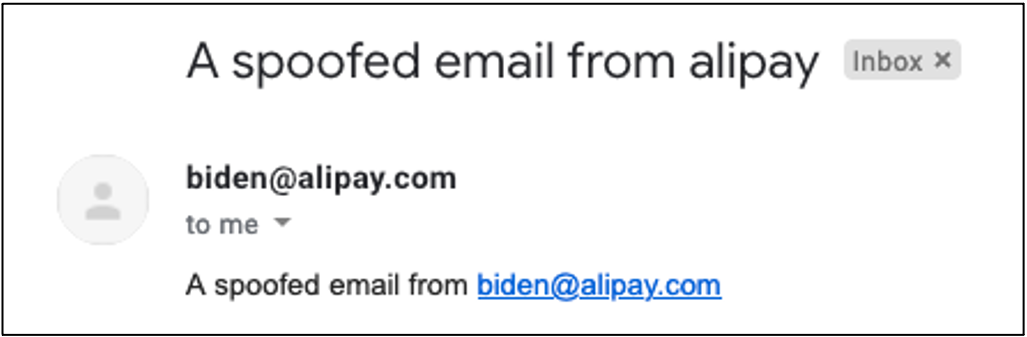
\includegraphics[width=\columnwidth]{graphs/ss_gmail_via_outlook.png}}
  \centering
  \caption{Email spoofing \dns{biden@alipay.com} via Outlook.}
  \label{fig:ss_gmail_via_outlook}
  \end{figure}


\begin{figure}[t]
  \centerline{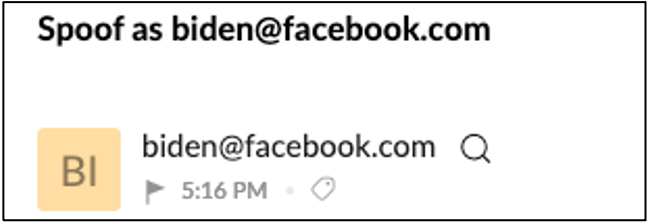
\includegraphics[width=\columnwidth]{graphs/ss_zoho_arc.png}}
  \centering
  \caption{Email spoofing \dns{biden@facebook.com} via Fastmail.}
  \label{fig:ss_zoho_arc}
  \end{figure}

\begin{figure}[t]
\centerline{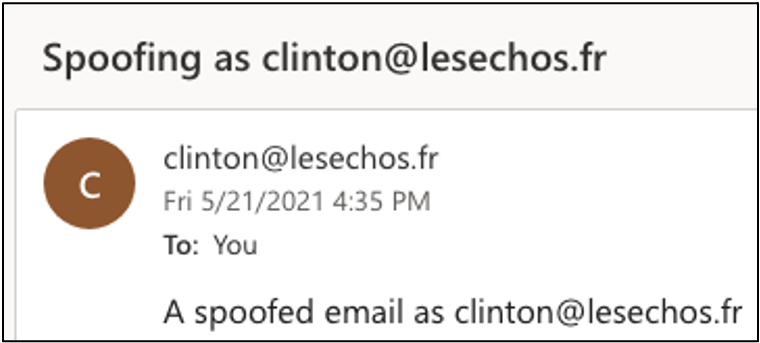
\includegraphics[width=\columnwidth]{graphs/ss_outlook_none.png}}
\centering
\caption{Spoofed email message taking advantage of Outlook's relaxed forwarding validation policy.}
% \geoff{let's see if Stefan notices this screenshot}}
\label{fig:attack_none_ms}
\end{figure}


\section{Additional Details for the Attack in Section~\ref{subsec:attack_zoho_arc}}
\label{sec:appendix_zoho_attack_details}
% \paragraph{Additional Details for the Attack in Section~\ref{subsec:attack_zoho_arc}}
Adversaries can broaden the scope of the attack described in Section~\ref{subsec:attack_zoho_arc} by using a forwarding
account at any email provider that Zoho trusts for ARC purposes,
including Gmail, and routing their spoofed email through multiple forwarding hops.
In particular, an attacker can obtain ARC headers in one forwarding hop via Gmail, and then bypass Gmail's lack of open forwarding by forwarding the email through a second account that does allow open forwarding (\eg, Outlook).
% The attacker can use a Gmail
% account to obtain the necessary ARC headers by including this account as an additional forwarding hop.
% For example, the attacker could create a second
% forwarding account on a platform that has open forwarding (\eg,
% Outlook).
For example, first, the attacker would send their spoofed email message
to their Gmail account, which they configured to forward to their
malicious Outlook account.
During the forwarding process Gmail will
attach a set of ARC headers to the email message.
Next, the spoofed email will arrive at their malicious Outlook account, which then forwards the email to any arbitrary Zoho recipient (because Outlook
supports open forwarding).
This forwarded email message will contain Gmail's attached ARC headers, enabling the attack to successfully pass DMARC validation checks as a result of Zoho's vulnerable ARC implementation.

Using our test accounts, I validated that this multi-hop attack variation
successfully delivers spoofed messages to the inbox of a Zoho recipient
without any warnings.






\section{Additional Details for the Attack in Section~\ref{subsec:attack_none_mailing_list}}
% \paragraph{Additional Details for the Attack in Section~\ref{subsec:attack_none_mailing_list}}
\label{sec:append_mailing_list_details}

% \subsection{Abusing Gaggle.email}

\begin{figure}[t]
\centering
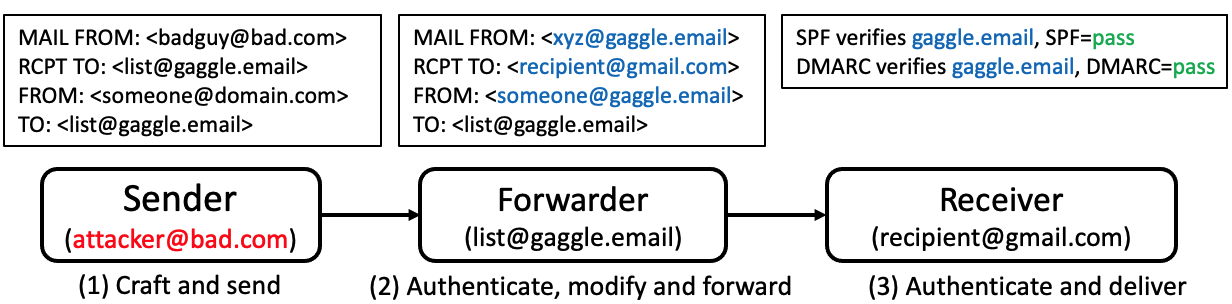
\includegraphics[width=\columnwidth]{graphs/mech_gaggle.png}
\centering
\caption{Attack flow for Gaggle.}
\label{fig:gaggle_email_mech}
\end{figure}

In addition to the attacks described in
Section~\ref{subsec:attack_none_mailing_list}, I found
additional attack variants related to Gaggle.
Figure~\ref{fig:gaggle_email_mech} shows an example of an attack that
abuses Gaggle's use of REM + MOD forwarding
(Section~\ref{sec:measure_forwarding_mechs_and_arc}). This attack works
regardless of the DMARC policy of the spoofed address's domain.  First, an
attacker chooses an address to spoof (\dns{someone@foo.com}) that is
allowed to send to a mailing list on a vulnerable provider
(\dns{list@gaggle.email}), and sends a spoofed email message
purporting to come from that address.  This spoofed email will fail
DMARC validation, but because Gaggle does not enforce DMARC
(Appendix~\ref{subsec:no_dmarc}), it will forward the email to the
mailing list's recipients as normal (Stage 2).  Since Gaggle uses a
REM + MOD forwarding process, it will rewrite the \textsc{MAIL FROM}
header to use the mailing list's domain (\eg, a
new \textsc{MAIL FROM} address of \dns{xyz@gaggle.email}).
%\grant{Similar to earlier, I should be more precise.}
Finally, when the spoofed email message arrives at the recipient's mail server,
it will properly pass SPF validation and DMARC alignment checks:
the rewritten \textsc{MAIL FROM} domain allows the mailing list to send on its behalf, and the domain matches the \textsc{FROM} address's domain (\dns{gaggle.email}).

% \subsection{Other Details}
% Below, I note one additional detail\alex{fix this number} about this attack.

Additionally, I note that mailing list software such as Listserv and
Mailman require a backend MTA.  In our experiments I used Postfix
with DMARC turned on, a configuration which follows good security
practice.  However, in practice many organizations might not use this
configuration because many MTAs (including Postfix) do not enforce
DMARC by default.  In these cases, the attacker can spoof email from any
target domain, regardless of its DMARC policy, much like the attack
against Gaggle.


%\section{Limitations}
%Most of the attacks described in this paper require that the attacker has an account on an email forwarding service and can configure the account to forward email message to the target account. Thus, massively and automatically performing the attacks described in this paper can be challenging. Automating the attacks (e.g., via automated account creation) is out of scope for this work.


\end{document}
